\documentclass{article}

\usepackage{microtype}
\usepackage{graphicx}
\usepackage{booktabs}
\usepackage{array}
\usepackage{hyperref}
\newcommand{\theHalgorithm}{\arabic{algorithm}}

% ICML 2027 version. The anonymous submission build defines \ANON before loading this file.
\ifdefined\ANON
\usepackage{icml2026}
\else
\usepackage[preprint]{icml2026}
\fi

\usepackage{amsmath}
\usepackage{amssymb}
\usepackage{amsthm}
\usepackage{xcolor}
\ifdefined\XeTeXversion\usepackage{fontspec}\setmainfont{texgyretermes}[Extension=.otf,UprightFont=*-regular,BoldFont=*-bold,ItalicFont=*-italic,BoldItalicFont=*-bolditalic]\setmonofont{texgyrecursor}[Extension=.otf,UprightFont=*-regular,BoldFont=*-bold,ItalicFont=*-italic,BoldItalicFont=*-bolditalic]\fi
\usepackage[capitalize,noabbrev]{cleveref}

\newtheorem{proposition}{Proposition}
\newtheorem{corollary}{Corollary}
\newtheorem{lemma}{Lemma}
% numbers that come from the preregistered held-out runs
\newcommand{\tbd}[1]{\textcolor{red}{[#1]}}

\icmltitlerunning{What moves the ceiling on automated audit}

\begin{document}

\twocolumn[
\icmltitle{What Moves the Ceiling on Automated Audit:\\
           from General Code to Scientific Code, Results and Data}

\begin{icmlauthorlist}
\icmlauthor{Zhaohe Dong}{ind}
\end{icmlauthorlist}

\icmlaffiliation{ind}{Independent researcher}
\icmlcorrespondingauthor{Zhaohe Dong}{dongzhaohe321418@gmail.com}

\icmlkeywords{code review, LLM critics, audit, evaluation, preregistration, AI for science}

\vskip 0.3in
]

\printAffiliationsAndNotice{}

\begin{abstract}
Audit benchmarks score an automated auditor against a hidden reference, yet on many cases the evidence the auditor
sees is equally consistent with the program and with the reference. For any flagging rule, recall minus false-flag
rate is then bounded by how well that evidence separates defective from correct programs, a classical testing fact
that audit evaluations cannot observe because a benchmark fixes one contract. We make it observable. From real
HumanEval+ and MBPP+ tasks we build execution-validated pairs of programs that differ only on a behaviour the task
leaves open, grade auditors against a contract drawn at random, and vary how the contract is revealed. On
\tbd{40} held-out units, with auditors from two vendors at two reasoning budgets, the auditors flag both programs
equally often when the contract is withheld, but diagnose departures from the benchmark's convention \tbd{y}
points more often than the reverse. Stating the missing requirement raises verified diagnosis by \tbd{z} points; a
higher reasoning budget changes it by \tbd{e}. Of 150 natural hidden-test failures, two model classifiers find that
the task's words single out the expected value in only 34, and solutions written from the task alone return the
``defective'' program's output about twice as often as the reference's. On scientific data, where the
documentation carries the information, a validator written from it captures nearly all that a model auditor
finds. What limits automated audit here is what the auditor is told, not how long it thinks. All held-out analyses
were preregistered.
\end{abstract}

% Draft (2026-11-07) for the ICML 2027 version. \tbd{} marks numbers from the preregistered held-out runs.
\section{Introduction}
\label{sec:intro}

MBPP+ problem 102 \citep{liu2023evalplus} asks for a function that converts a snake-case string to camel case and
gives three ordinary examples. A generated function splits on underscores, capitalises each word and passes
all three. The hidden suite then passes \verb|___python_program| and expects \verb|___PythonProgram|; the function
returns \verb|PythonProgram|. The task says nothing about how to handle leading underscores. The benchmark treats
this program as defective. By that measure, an automated auditor that reads and passes it has missed a defect.

Models increasingly check what other models write. Audit benchmarks score them as in this example, against a hidden
reference. We argue that these scores conflate two kinds of case. In some, the evidence available to the auditor
determines the correct behaviour, and a miss is the auditor's failure. In others, such as the example above, the
evidence is equally consistent with the program and the reference; where the evidence is moreover identically
distributed under both behaviours, as our construction guarantees, no auditor, whatever its capacity, can tell them
apart without being told which behaviour is wanted. A ``detection'' in these cases amounts to agreement with the
benchmark's convention; it would be a false accusation had the convention gone the other way.

This distinction is classical. For any flagging rule, recall minus false-flag rate is bounded by the total
variation between the evidence a defective and a correct program produce. The best attainable recall at a given
false-flag rate is the Neyman--Pearson power of that evidence (Section~\ref{sec:framework}). Audit evaluations have
lacked a way to observe this distinction because a benchmark fixes one contract and hides the counterfactual.
We construct that counterfactual experimentally (Section~\ref{sec:e6}). Each unit starts with a real benchmark task
that leaves one behaviour open; we build two programs that differ only in that behaviour. We grade the auditor against a
contract drawn independently of what it sees, then reveal the contract in different ways. Execution validates the
programs, oracles and boundaries of the open behaviour; two models, which also implement the rules, judge whether both are admissible.

\textbf{Findings.} Across \NSixUnits{} held-out units and auditors from two vendors at two reasoning budgets:
\begin{itemize}\itemsep1pt
\item With the contract withheld, flagging cannot track which program is wrong: the same readings are scored under
  both contracts, so recall equals the false-flag rate (\NSixNoneFlag\%) by construction. The informative difference
  is which program is flagged. The one that departs from the benchmark's behaviour is flagged \NSixFlagPref{} points
  [\NSixFlagPrefLo, \NSixFlagPrefHi] more often than the one that follows it, and diagnosed more often too (the registered convention advantage, half
  the difference between the two diagnosis rates, is \NSixTwo{} points [\NSixTwoLo, \NSixTwoHi]).
\item The models' own solutions written from the task alone follow the benchmark's behaviour on these units 89\%
  of the time. The convention the benchmark rewards is one the models share, and rewarding it would be a false
  accusation had the task's author meant the other rule.
\item Adding the missing requirement as one ordinary sentence raises verified diagnosis by \NSixFive{} points
  [\NSixFiveLo, \NSixFiveHi] over the task alone, with no correct program flagged in that arm (\NSixResolveFpr\% when the contract is
  stated as a choice between the two rules).
\item When told only that the task leaves the choice open, the two vendors respond differently: one passes almost
  every program, while the other asks for clarification.
\item On positive controls, where the task's words rule out one program, the same auditors separate the programs
  without being told (recall minus false-flag rate \NSixFourJ{} points).
\end{itemize}
Among natural hidden-test failures (Section~\ref{sec:natural}), fewer than a quarter are ones that both classifiers
agree the task's words determine. Three earlier preregistered studies of scientific code, results and data
(Section~\ref{sec:transfer}) are consistent with the same distinction, although none of them varied the information
an auditor receives in the way our experiment does.

\textbf{Contributions.} (i) A randomised-contract design that makes the information limit of an audit observable and
separates convention agreement, unjustified accusation, requests for clarification and verified diagnosis, with
execution-validated programs and oracles. (ii) Preregistered evidence that, on such cases, auditors side with the benchmark's convention, and that one
added sentence stating the requirement turns that agreement into verified diagnosis. (iii) A description of
natural hidden-test failures by whether the task's words determine the expected value, and an
interpretation of scientific code, results and data audits using the same distinction between capacity and information misses.
Code, records and preregistrations are released.

% Draft (2026-11-07): the evidence ceiling. To be revised after GPT review round P2.
\section{The ceiling is a property of the evidence}
\label{sec:framework}

\paragraph{Setting.}
An audit case consists of a program $X$, the evidence $E$ shown to the auditor (the task text, the visible tests,
any added text, and anything the auditor can compute from these, including by executing $X$), and a hidden
contract $H$ that defines the ground truth. The program is defective, $D=1$, if it violates $H$. An auditor is any
measurable, possibly randomised, map from $E$ to a flag; we write $\phi(e)=\Pr(\text{flag}\mid E=e)\in[0,1]$.
Sampling more readings, using a larger model, reasoning longer or executing the supplied code changes $\phi$ but not
the joint law of $(E,D)$. Write $P_1$ and $P_0$ for the laws of $E$ given $D=1$ and $D=0$.

\begin{proposition}[Evidence ceiling]
\label{prop:ceiling}
For every auditor $\phi$,
\[
\mathrm{TPR}(\phi)-\mathrm{FPR}(\phi)\;\le\;\mathrm{TV}(P_1,P_0),
\]
and for every $\alpha\in[0,1]$, $\max\{\mathrm{TPR}(\phi):\mathrm{FPR}(\phi)\le\alpha\}$ is attained by a
likelihood-ratio test of $E$, so the receiver operating characteristic of the likelihood ratio is the ceiling for
all auditors that see $E$.
\end{proposition}

\begin{proof}
$\mathrm{TPR}-\mathrm{FPR}=\int\phi\,(p_1-p_0)\,d\mu\le\int_{p_1>p_0}(p_1-p_0)\,d\mu=\mathrm{TV}(P_1,P_0)$ for
densities $p_1,p_0$ with respect to a dominating measure $\mu$, since $0\le\phi\le1$. The second statement is the
Neyman--Pearson lemma.
\end{proof}

\begin{corollary}[Indistinguishable component]
\label{cor:component}
Suppose the cases split into components and, on a component $K$, $E$ has the same law for defective and correct
programs. Then every auditor has $\mathrm{TPR}_K=\mathrm{FPR}_K$. If a share $\pi$ of the defects lies in such
components, recall at component false-flag rate at most $\alpha$ is at most $(1-\pi)+\pi\alpha$.
\end{corollary}

Both statements are textbook facts about hypothesis testing (the Neyman--Pearson lemma and the total-variation
bound on any test's power minus its size; \citealp{neyman1933efficient}); we claim no novelty for them. Note that the
component bound needs the false-flag constraint on the component itself: under an overall false-flag rate $\alpha$
alone, with $q$ the share of correct programs in the component, the bound is only $(1-\pi)+\pi\min(1,\alpha/q)$.
Their use here is to separate two causes of a missed defect that audit evaluations conflate. A miss on a distinguishable case is a \emph{capacity} miss: some auditor with the same evidence could do
better. A miss on an indistinguishable case is an \emph{information} miss: no auditor can do better without
different evidence. Only interventions that change $E$ move the ceiling.

\paragraph{Contract randomisation makes the component observable.}
On a natural benchmark the hidden contract is fixed to the benchmark's reference behaviour, so indistinguishability
is a counterfactual: we cannot see the auditor's response under the other admissible contract. We construct it.
Take a discrepancy unit: an input class on which two behaviours, $A$ and $B$, are both admissible under the task
text and the visible tests. Build two programs that differ only on that class, $X_A$ and $X_B$, and draw
$H\in\{A,B\}$ independently of everything the auditor sees.

\begin{lemma}
\label{lem:symmetric}
If $E$ depends on $(X,H)$ only through $X$ and $H$ is independent of $X$ with $\Pr(H=A)=\tfrac12$, then $P_1=P_0$ on
the unit, so every auditor's recall equals its false-flag rate, whatever its capacity.
\end{lemma}

\begin{proof}
With $X$ uniform over $\{X_A,X_B\}$, $D=1$ exactly on $(X_A,B)$ and $(X_B,A)$ and $D=0$ on $(X_A,A)$ and $(X_B,B)$.
Each event has probability $\tfrac14$, and the law of $E$ given each depends only on $X$, so $P_1=P_0=\tfrac12
Q_{X_A}+\tfrac12 Q_{X_B}$, where $Q_x$ is the law of $E$ given $X=x$.
\end{proof}

Revealing $H$ in the evidence (stating the requirement) breaks the premise of Lemma~\ref{lem:symmetric}; text that
draws attention to the input class, or lists both behaviours without choosing, does not. The experiment in
Section~\ref{sec:e6} therefore measures three things that the propositions leave open: how far real auditors sit
below the ceiling once the requirement is revealed, whether additional computation helps more before or after
the reveal, and how much of the recall measured on natural benchmarks is agreement with the benchmark's convention
on indistinguishable units, which would be false flags had the convention gone the other way.

\paragraph{What we do not claim.}
The ceiling is relative to the evidence, and the evidence includes what a model brings with it: a model that has
memorised a benchmark's reference sees more than the task text. Contract randomisation neutralises this on the
constructed units, because the memorised convention is equally likely to be wrong. On natural units we can only
bound the information-limited share using human judgements of admissibility, which we report with their agreement.

% Draft (2026-11-07). Test numbers are marked \tbd{} until the preregistered test run.
\section{A randomised-contract audit experiment}
\label{sec:e6}

Section~\ref{sec:framework} says that a miss on an indistinguishable case cannot be repaired by computation, but
on a natural benchmark we never observe the counterfactual contract. This section builds it. Each unit is a real
benchmark task with one behaviour the task leaves open; we write two programs that differ only there, draw the
contract the auditor is graded against independently of what it sees, and then reveal the contract, or not.

\subsection{Construction}
\label{sec:e6-construction}

\paragraph{Contracts first.} For each of the 542 HumanEval+ and MBPP+ problems \citep{liu2023evalplus}, a proposer
model names one kind of valid input on which the task text and the visible tests leave the behaviour open, and states
two rules for it as requirements a task author could add: \emph{B}, the behaviour the benchmark reference follows,
and \emph{A}, an alternative of equal specificity (for example, ``if several sublists are equally short, return the
first'' against ``\dots the last''). Each rule is then implemented from the task and the rule alone, by two vendors
with the same prompt; no implementation sees the reference. The programs an auditor reads are one vendor's A and B
implementations, so the two share provenance and style; the vendor alternates across units.

\paragraph{Admission by execution.} An independent model writes a domain predicate \texttt{valid} and 16--24 probe
inputs; the proposer writes a class predicate \texttt{in\_class}. A unit is admitted only if, on every valid input
among the hidden suite, the proposer's inputs, the probes and 120 seeded stress mutations (unusual whitespace and
Unicode, extreme and cancelling floating-point values, empty and duplicated collections), both B implementations agree with the reference; outside
the class all four implementations agree with the reference; inside it the two A implementations agree; A and B
differ on at least two valid class inputs; and every implementation passes the visible tests. Each stage is attempted
once per problem; problems without a first-attempt primary unit received one second, independent attempt, fixed
before any held-out audit. These checks reject,
for example, a ``correct'' B program whose integer summation silently became floating point.

\paragraph{Judging without human raters.} Two models that neither proposed the rules nor audit (Claude Opus,
GPT-6.1-sol) judge, blind to which rule is the benchmark's, whether the inputs are valid and whether each rule is
compatible with the task's words and visible tests, with the instruction that a missing example is not permission.
The primary population is the admitted units on which both judges accept the domain and both rules. We call these
\emph{execution-validated, two-model-compatible contract pairs}. They are not human-validated ambiguities, and we make
no claim about how common such ambiguity is.

\paragraph{Positive controls.} The same pipeline, with a proposer prompt asking for a plausible \emph{misreading}
that passes the visible tests but that the words rule out, yields units on which the evidence does distinguish the
programs. Both judges must call the misreading incompatible and the required rule compatible.

\subsection{Arms, auditors and scoring}
\label{sec:e6-arms}

Each open unit is audited under six arms that append text to the task: nothing (\textsc{none}); both rules as a
numbered menu with the statement that the task does not say which applies (\textsc{menu}); the same menu plus
``the function must follow rule ($k$)'' (\textsc{resolve}); and one rule stated as an ordinary requirement with no
menu (\textsc{sentence}). Menu order is fixed per unit and independent of the contract. Auditors are GPT-5.6-terra and
Claude Sonnet 5.5, each at a low and a high reasoning budget, with the shipped rulebook and two readings per cell
(\tbd{N} readings in all).

Under contract $X$, program $X$ is correct and the other is defective. In \textsc{none} and \textsc{menu} the evidence
does not depend on the contract, so the same readings are scored under both contracts (Lemma~\ref{lem:symmetric}
then forces flag recall to equal the false-flag rate; we report it as a check). A cell flags if either reading
reports a blocking finding. A diagnosis is \emph{verified} only if a flagging reading supplies a witness call that
satisfies \texttt{valid}, lies in the class, and on which the program and the contract's oracle disagree under the
benchmark's own comparator (the reference for B, the other vendor's implementation for A), and both judges confirm
that the witness exercises the disagreement. A unit's value is the mean over configurations; intervals are
problem-level bootstraps, and the false-flag budget after resolution (10\%) is tested separately with a betting
confidence bound \citep{waudbysmith2024betting}, which does not gate the other claims.

% Draft (2026-11-07). \tbd{} marks numbers from the preregistered E1 test run.
\section{What natural audit failures are made of}
\label{sec:natural}

The randomised experiment isolates the information limit on constructed units. We ask how much of an ordinary audit
benchmark is subject to that limit. We use 150 programs written by two generator models for HumanEval+ and MBPP+
problems. Each program passes its visible tests but fails the hidden suite and is paired with a test-passing control
\citep{liu2023evalplus}.

\paragraph{Most hidden-test failures are not determined by the task.} Two models classify each program's first failing
input, blind to which output is the benchmark's (order randomised by evidence). The categories are: the input is
outside the task's domain, only the reference's output is acceptable (\textsc{determined}), both are
(\textsc{open}), only the program's is (\textsc{at odds}), or neither. Identical evidence is pooled so that it cannot
receive two labels. Of the 150 failures, 34 are \textsc{determined}, 26 \textsc{open}, 37 \textsc{at odds},
21 out of domain and 32 disputed (Cohen's $\kappa=0.78$ on the 43 development items). Only on 34 of the 150 (23\%) do
both classifiers agree that the task's words single out the value the hidden suite expects; on 63 they agree that
the words leave it open or point the other way.

\paragraph{Other solutions mostly side with the ``defective'' program.} A behavioural check avoids classifier
judgement. For each failure, two generators wrote twelve solutions from the task alone; we run the 1{,}710
of the 1{,}800 that pass the visible tests on the same first failing input. They return the defective program's
result 1{,}080 times and the reference's 559 times (71 neither); for 93 failures most solutions side with the
defective program, for 46 with the reference. The solutions come from the same two generators that wrote the failing
programs, so this is partly a model agreeing with itself; still, on the inputs that define these programs as
defective, the benchmark's expected value is the minority reading among solutions written from the task. The
behaviour also checks the classification (Figure~\ref{fig:natural}b): where the classifiers judge that only the
program's output fits the words (\textsc{at odds}), 90\% of independent solutions return it; where they judge the
reference's value determined, solutions split almost evenly, which is consistent with defects the generators commonly
share.

\begin{figure}[t]
\centering
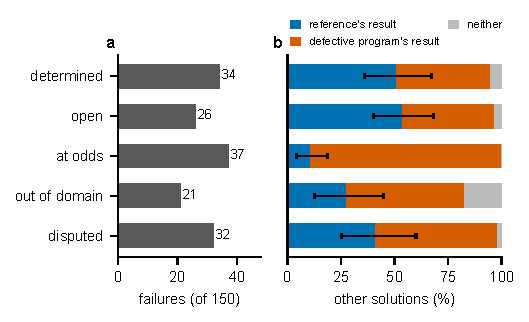
\includegraphics[width=\columnwidth]{fig_natural.pdf}
\caption{Natural hidden-test failures (150 programs that pass their visible tests). (a) Class of the first failing
input, as two classifiers judge it from the task's words and visible tests, with identical evidence pooled. (b) What
independent solutions written from the task alone (and passing the visible tests) return on that input, by class;
the interval is an item-level bootstrap for the share returning the reference's result.}
\label{fig:natural}
\end{figure}

\paragraph{What auditors verify.} With the original task text, four readings per program and two auditors, verified
diagnosis on the held-out failures is \NOneVdDetermined\% on \textsc{determined} failures and \NOneVdOpen\% on
\textsc{open} ones. The registered contrast (H6) is \NOneHSix{} points [\NOneHSixLo, \NOneHSixHi] and is not
supported: on these failures the class of the first failing input does not predict whether an auditor verifies a
defect (the development estimate, from 13 items, was 50 points). The witnesses tell a more specific story. Of the
\NOneBridgeItems{} held-out programs with a verified diagnosis, \NOneBridgeDetermined{} have at least one witness that
both classifiers label \textsc{determined}: an auditor that verifies a defect in an \textsc{open} failure usually does
so through a different input, on which the words do decide. Hidden-test recall on such a benchmark therefore mixes
two things: on behaviour the words determine it measures the auditor, and elsewhere it measures at best agreement
with a convention the task does not state. The classification concerns the first failing input only, so a program
may also have determined defects elsewhere.

\paragraph{Clarifying the missing requirement.} For the 13 failures that remain \textsc{open} after reclassification
and whose added sentences pass a neutrality recheck, we appended the missing requirement as one sentence, a
length-matched placebo, or a pointer naming the input class without resolving it. The \NOneItems{} held-out items
(\NOneProblems{} problems) provide a small replication of Section~\ref{sec:e6}: the clause raises verified
diagnosis by \NOneHOne{} points [\NOneHOneLo, \NOneHOneHi] over the placebo (H1) and by \NOneHFive{} points
[\NOneHFiveLo, \NOneHFiveHi] over the pointer (H5), and the placebo does nothing (H4). Whether the clause also
raises flags on correct programs could not be settled at this size (H2: $-$5.6 points [$-$33.3, 22.2]).

% Draft (2026-11-07). E3 numbers are final (preregistered, Amendment 3).
\section{Transfer: auditing scientific data}
\label{sec:data}

For data, the information an auditor needs is in the documentation: units, ranges, what a row is. We asked whether a
model auditor adds anything to a validator written mechanically from that documentation. Twelve public regression
datasets were each delivered with a data card and either left clean or given one injected fault (mixed units,
negated values, duplicated rows, a shuffled target, swapped columns, sentinel values, rounding); four datasets were used for
development and eight held out. A profile validator derived from the card was combined with one of two auditors,
GPT-5.6-terra or Claude Sonnet 5.5, run either with a shell on the full table or reading a 120-row table with every
tool disabled. Faults counted as localised only if a blocking finding names the injected fault type and column,
scored by code against the injection manifest.

\paragraph{Isolation.} An auditor with a shell can look for the clean source instead of auditing the table. In an
earlier run the GPT auditor searched the disk and the web for the original UCI files and found copies kept for item
construction; we discarded that run. Every reported reading runs inside an operating-system sandbox that denies reads
outside the reading's own copy of the item and all network except the vendor's API. Inside it, 57\% of the GPT
auditor's held-out readings (86\% in development) still attempted out-of-scope access, against none of Claude's; the
attempts are logged and could not return information.

\paragraph{Results (held out, 266 items, preregistered).} Adding the model to the card-derived validator raised
correct localisation by 2.3 points [0.4, 4.8] and flags on clean items by 16.0 points [3.2, 31.4], above the
registered tolerance of 10. Neither the full 12{,}000-row table (0.0) nor tool use over reading (+1.3 [$-$2.7, 5.8])
helped. Where the documentation already carries the information, a validator written from it captures nearly all of
what the model finds, and the model's additional contribution is mostly false alarms.

\section{Related work}
\label{sec:related}

\textbf{Critics and repeated reading.} Trained critics catch more bugs in model-written code than unaided humans
and hallucinate some \citep{mcaleese2024critics}; aggregating review passes raises review F1 on real pull requests
\citep{zeng2025swrbench}; coverage under repeated sampling grows roughly log-linearly in the number of samples
\citep{brown2024monkeys}; and self-correction without external feedback does not reliably help
\citep{huang2024selfcorrect}. These results vary the auditor while holding the evidence fixed. We vary the evidence
while holding the auditor fixed, and show that on the cases we construct the second moves performance and the first
does not.

\textbf{What the hidden suite decides.} EvalPlus rebuilt HumanEval and MBPP with larger suites
\citep{liu2023evalplus}; models collapse onto one reading of an underspecified task \citep{richter2026collapse};
generated tests err mostly in the expected value \citep{xiong2023testing}; and generated oracles capture what a
program does rather than what was intended \citep{konstantinou2024oracles}. Label errors in test sets bound and
reorder what benchmarks can measure \citep{northcutt2021labelerrors, gema2025mmlu}. Our setting differs: the
reference is not wrong, it is one of several behaviours the task admits, so the right correction is neither
relabelling nor discarding but stating the contract, and we measure what stating it does.

\textbf{Clarification.} Code generators can be made to ask clarifying questions when a task is ambiguous
\citep{mu2024clarifygpt, wu2025humanevalcomm}, or to formalise intent as tests confirmed by a user
\citep{lahiri2022ticoder}; abstaining when evidence is insufficient is the classical reject option
\citep{chow1970reject}. We study the auditing side: we score a request for clarification as a separate outcome,
neither a detection nor a pass, and find % CHECK against held-out routing result
 that the two vendors' auditors differ sharply in how often they make one.

\textbf{Auditing scientific work.} Models detect a minority of errata-grade errors in manuscripts
\citep{son2025spot} and of paper--code discrepancies \citep{baumgartner2026scicoqa}; an auditor of AI-scientist
projects detects pitfalls far better with logs and code than with the paper alone \citep{luo2025pitfalls}; cleaning
agents miss errors that span rows \citep{bendinelli2025cleaning}; and an expert audit of SciCode
\citep{tian2024scicode} found specifications and tests that reject correct solutions \citep{hu2026scicodeverified},
which it repairs by rewriting the specification. Our randomised contracts are the experimental counterpart of that
repair: they measure how much of an auditor's apparent miss rate a repaired specification would remove.

\textbf{Statistics.} The ceiling is the Neyman--Pearson bound \citep{neyman1933efficient}; the false-flag budget is
tested with a betting confidence sequence \citep{waudbysmith2024betting}, which is valid at any sample size.
Preregistration of evaluations is beginning to appear in machine learning \citep{vaccaro2026prereg,
thomas2026phacking}; here it is method, not contribution.

\section{Discussion and limitations}
\label{sec:discussion}

\paragraph{Interpretation.} On units where the task leaves a behaviour open, a hidden-test ``detection'' is
agreement with the benchmark's convention, and the auditors we tested agree with it more often than chance
(Section~\ref{sec:e6}). Adding one sentence that states the convention turns that agreement into verified
diagnosis. A larger reasoning budget does not. Natural failures show the same pattern without construction.
The task's words do not settle most failures, and independent programmers mostly behave like the ``defective''
program. The diagnoses auditors do verify concern what the words settle (Section~\ref{sec:natural}).
Scientific work shows both sides of this distinction (Section~\ref{sec:transfer}). Naming the deliverable cut
false flags on correct scientific code from 69\% to 36\%. Where code and inputs determine a reported value,
recomputation by the model, or by re-execution, catches fabrications that consistency checks cannot.
Where documentation states what valid data look like, a validator written from it already finds most faults.
Computation helps where the evidence decides; elsewhere the ceiling moves with what the auditor is told.

\paragraph{Practical consequences.} Alongside recall, an audit benchmark should report which of its cases the
task determines. It should not count agreement with an unstated convention as detection. An auditor that is
unsure whether a behaviour is required should be scored for asking, not only for flagging or passing.
Writing down the missing requirement is the cheapest deployment improvement we measured.

\paragraph{Limitations.}\label{sec:limits} \emph{Constructed units.} The randomised-contract units are execution-validated;
two models, rather than people, judge them admissible. We make no claim about how often such ambiguity occurs.
Agreement between two models that a rule is compatible with a task is weaker than expert agreement.
\emph{Benchmarks.} All randomised-contract and natural-failure units come from HumanEval+ and MBPP+, short functions with small specifications.
Whether the size of the convention advantage carries over to larger programs, where more behaviour is
unstated, remains untested. \emph{Auditors.} We tested two vendors' models at two reasoning budgets with one rulebook.
Other auditors, agent scaffolds or execution-based test generation may sit closer to the ceiling before the
reveal, although Lemma~\ref{lem:symmetric} bounds what any of them can do on the unrevealed arms.
\emph{Verification.} A verified diagnosis requires a witness that the benchmark's own comparator confirms and
two judges accept. We do not credit diagnoses stated only in prose, which can understate auditors whose
findings are correct but unexecutable. \emph{Natural failures.} Models classify the natural failures, with
Cohen's $\kappa$ of 0.78 on development items. The behavioural check uses solutions from two generators only.
\emph{Data.} The data study injects one fault per item into twelve public tables; its conclusion is specific to
faults that documentation describes. \emph{Earlier studies} of the shipped configuration
(Appendix~\ref{app:earlier}) are reported as registered and are not re-analysed here.


\section*{Impact Statement}
This paper concerns how much automated auditors of model-written code and data should be trusted. It argues
against reading a hidden-test recall figure as auditor capability when the task does not determine the expected
behaviour, and against counting agreement with a benchmark's convention as detection. A risk is that the
constructed units are used to tune auditors toward a benchmark's conventions; we release them with both contracts
for that reason. All data are public benchmarks and datasets under permissive licences; no human subjects were
involved.

\bibliography{paper}
\bibliographystyle{icml2026}

\newpage
\appendix
\onecolumn
\section{Earlier studies of one shipped audit configuration}
\label{app:earlier}
\section{The system under study}
\label{sec:system}

Every auditor reading in this paper is taken through one shipped system, CrossAudit. Every auditor
prompt is built by the product's own prompt builder, and every family but one is read through
the product's own audit call; the exception, \texttt{gpt-6-astra}, receives the same prompt
bytes through a direct call. We describe the system first because
its design fixes what the later sections can and cannot vary. We state its structure only here
and quote no measurement of it. Its limits are the subject of
Section~\ref{sec:ceiling} onward.

\textbf{Separation of roles.} A generator model writes an increment (a set of files) into a Git
repository. An auditor model then reads the committed bytes and returns findings, each graded
BLOCKER or ADVISORY. The auditor must come from a different vendor from the generator: the audit
refuses to run when the configuration names the same vendor for both roles, and when the
generator's vendor is not declared, the receipt records that independence could not be asserted.
The same-vendor arms below run with the generator's vendor undeclared, deliberately. The premise is that a model
reviewing its own vendor's output is an interested reader. The product takes that premise as given, and Section~\ref{sec:ceiling} puts
one consequence of it to the test: whether a same-vendor auditor catches more or less.

\textbf{Two tiers of evidence.} Before the auditor reads anything, a deterministic check layer
runs registered checks over the same committed bytes. A check's finding is \emph{verified}: code
produced it and code can reproduce it. A model's finding is \emph{raised}: it is a reading, not
yet reproduced. The checks are grouped into named profiles, so strictness is a setting the
project chooses:
\begin{itemize}\itemsep0pt
\item \texttt{general}, the default: structured files parse, every local path a file lists as an
  input or dependency exists, and relative links and leftover placeholders are reported as
  advisory.
\item \texttt{science}: results carry a schema; quantities carry units; a result that reports
  convergence must meet its own threshold; every input a result depends on is listed, exists and is cited at an exact revision
  (\emph{provenance}); and every number a report states is annotated with the file and quoted span
  it came from, which a check matches against the cited bytes (\emph{number$\to$source}).
\item \texttt{research}: the general profile's checks plus a citation check under which a report may cite only
  sources it fetched through a governed tool.
\end{itemize}
The science profile follows one rule throughout, and the rule is the one Section~\ref{sec:ai4s} tests: \emph{the
model names its evidence, and code verifies it.} A number with no source line, a unit that
disagrees with its schema or an input that does not exist fails without any model's opinion.

\textbf{Computed verdicts.} The verdict is derived by code from the evidence, in a
fixed order. A failed deterministic check blocks, whatever the model says. A model BLOCKER with
no deterministic support either blocks or escalates to a person, according to a project setting.
A blocked increment goes back to the generator for a bounded number of revision rounds, three by
default. Each revision passes a repair guard before it is committed: an edit outside the audited
scope is refused, and a new catch-all handler, a deleted assertion or a skipped test is flagged to
the auditor for the next round.

\textbf{Receipts.} A passing round produces a receipt that binds the verdict to the commit that was
audited, the commit of the rulebook the auditor was given, and a digest over every finding with its
tier. Every model call is written to a ledger with its prompt hash and cost. A verification command
recomputes the digest from the recorded evidence, so a receipt can be checked by someone who does
not trust the operator.

\textbf{What the rest of the paper measures.} Section~\ref{sec:ceiling}, with
Appendices~\ref{sec:method} and~\ref{sec:results}, measures the model tier on its own. There, an
increment counts as flagged when the auditor grades any finding BLOCKER, and the general profile's
checks run as in the product but decides no recall or false-positive outcome. The model tier is the
part of the system whose limit is least known, since a deterministic check catches exactly what it
was written to catch. Section~\ref{sec:ai4s} measures the model tier on scientific code, and sets
it beside deterministic verification on reported results and on data, asking what each flags that the
other does not.

\section{The ceiling on general-purpose code}
\label{sec:ceiling}

\textbf{Substrate and ground truth.} HumanEval+ and MBPP+ \citep{liu2023evalplus}: Python functions
with an executable hidden test suite. One frozen generator (\texttt{claude-haiku-4-5}) was shown each
specification and its visible tests and wrote one solution per problem, over two passes of 540
problems. A candidate that passes the visible suite and fails the hidden one is \emph{defective}; one
that passes both is \emph{correct}. Recall is measured on all 110 defective instances (56 problems)
and false positives on 150 correct ones drawn by seed. The auditor sees the specification, the
visible tests and the candidate, never the hidden suite. Because the defective stratum already
survived the visible tests, recall here is the fraction of that harder subset caught, not of all
defects a model writes (Appendix~\ref{sec:method}).

\textbf{Estimand and statistics.} Union recall at $K$: the fraction of defective instances blocked
(any finding graded BLOCKER) by at least one of $K$ independent readings, averaged exactly over all
size-$K$ subsets of the readings. The same union on correct instances is the false-positive rate,
always reported beside it (Table~\ref{tab:primary} collects the primary quantities). Intervals are 95\% problem-cluster percentile bootstraps; paired contrasts
carry exact McNemar and cluster sign-flip tests. The shipped cross-vendor route
(\texttt{gpt-5.6-terra}) sends no sampling parameter; same-vendor routes are sent temperature 0, a
difference that bounds every cross-family union contrast (Section~\ref{sec:auditor}).

\begin{figure*}[t]
\centering
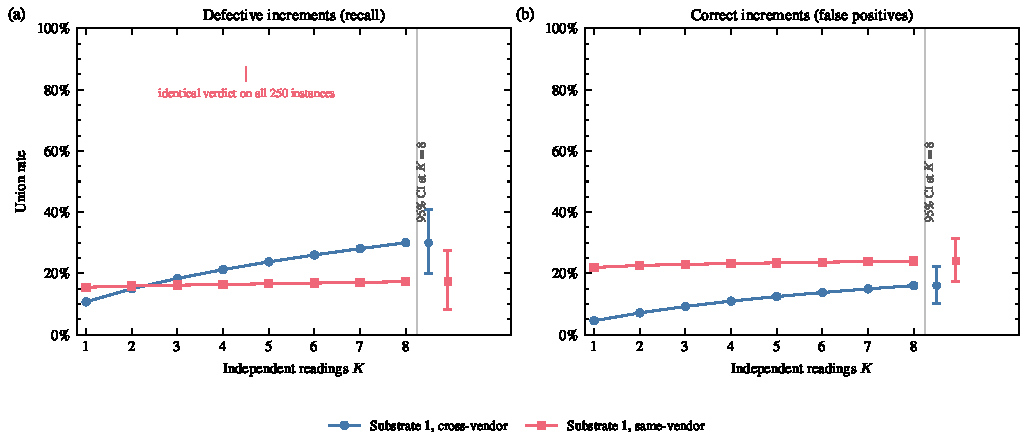
\includegraphics[width=\textwidth]{fig1_saturation.pdf}
\caption{\textbf{Returns to repeated reading diminish short of complete.} Union rate against the
number of independent readings $K$, for two auditor families. (a) Recall on defective instances;
(b) false positives on correct instances. Bars at the right of each panel give the 95\%
problem-cluster bootstrap interval of each series at $K=8$, dodged in $x$ so overlapping intervals
stay separable. The cross-vendor curve does not meet the preregistered flattening bar (its
last-step gain is 1.93 points [1.14, 2.78] against a bar of 1.0) and is not described as
saturating. The same-vendor curve meets it, at 0.23 points, but that route is sent temperature
$0$ and its verdict varies across readings on only 3 of 110 defective instances under this
configuration, so its flatness is not evidence of exhausted headroom; whether it reflects the
sampling or the model is not separated here (Section~\ref{sec:auditor}).}
\label{fig:saturation}
\end{figure*}

\begin{table*}[t]
\caption{Every primary quantity this paper quotes, with the population it is measured on and the label its source report gives it. Values are percentages or percentage points. Intervals are 95\% problem-cluster percentile bootstraps unless the label names another method. The coverage simulation of \S\ref{sec:stats} measures single-rate intervals only; the contrasts and the category-conditioned shares have no measured coverage. Every row is read from a committed record by \texttt{figures/make\_table1.py}.}
\label{tab:primary}
\centering
\footnotesize\setlength{\tabcolsep}{4pt}
\begin{tabular}{@{}llrll@{}}
\toprule
quantity & population & value & interval & label \\
\midrule
Union recall, shipped route, $K=8$ & 110 defect, 56 problems & 30.0\% & $[20.0, 40.7]$ & preregistered \\
Union false positives, shipped, $K=8$ & 150 correct, 143 problems & 16.0\% & $[10.1, 22.3]$ & preregistered \\
Pooled union, 3 routes & 110 defect & 48.2\% & $[36.7, 60.0]$ & preregistered \\
Gain from the eighth reading & 110 defect & $+1.93$ & $[1.14, 2.78]$ & bar 1.0, not met \\
Same-vendor stronger $-$ cross, recall & 110 defect & $-26.4$ & $[-37.3, -15.6]$ & preregistered \\
\quad its false-positive difference & 150 correct & $-12.7$ & $[-19.3, -6.1]$ & prereg.; 3.3\% v 16.0\% \\
Rulebook rule $-$ shipped, recall & 110 defect & $+30.9$ & $[+19.1, +43.1]$ & preregistered \\
\quad its false-positive cost & 150 correct & $+20.7$ & $[+12.8, +28.8]$ & preregistered \\
Rulebook rule, flags & 56 loop defect & $+26.8$ & $[+13.6, +40.4]$ & exploratory \\
\quad its cost on correct code & 56 loop correct & $+12.5$ & $[-3.6, +26.8]$ & exact unconditional \\
\quad isolating contrast, pass rate & 112 loop, 96 problems & $+5.4$ & $[-0.9, +12.1]$ & registered, failed \\
\texttt{astra} $-$ cross, common $K=4$ & 110 defect, 56 problems & $+11.5$ & $[+2.9, +21.3]$ & exploratory \\
\quad its false-positive difference & 150 correct & $-0.3$ & $[-3.8, +3.4]$ & exploratory \\
Undetermined, sheet groups & 121 entries, 110 instances & $+19.8$ & $[+1.2, +38.1]$ & registered method \\
\quad one definition of caught & 57 against 53 & $+23.3$ & $[+2.0, +43.6]$ & post hoc \\
Undetermined share, 3-family residual & 44 of 57 & 77.2\% & $[62.1, 91.1]$ & post hoc \\
\quad 6-family residual & 25 of 32 & 78.1\% & --- & post hoc, pending \\
Clarified $-$ original, diagnosis & 32 selected, 19 problems & $+28.1$ & $[+7.7, +51.4]$ & one-signed; exact $p$ .0625 \\
\bottomrule
\end{tabular}
\end{table*}


\textbf{Repeated reading.} Union recall rises from 10.7\% at one reading to 30.0\% [20.0, 40.7] at
eight, at 16.0\% [10.1, 22.3] on correct code (Figure~\ref{fig:saturation}). The eighth reading still
adds 1.93 points [1.14, 2.78], above the 1.0-point flattening bar registered in advance, so we report
diminishing returns, not saturation. Twenty readings pooled across three families reach 48.2\%
[36.7, 60.0] at 36.0\% [28.2, 44.2] on correct code: pooling buys coverage at its own price.

\textbf{Which model reads.} Replacing the auditor with a stronger same-vendor model moved union
recall at eight readings by $-26.4$ points [$-37.3$, $-15.6$] (exact McNemar $p = 4.2\times10^{-7}$; cluster sign-flip $p = 2.0\times10^{-5}$),
a preregistered primary. It does not measure auditing ability. The stronger model flags 3.3\% [0.7, 6.7] of
correct code against 16.0\%; under an exploratory any-finding rule the sign reverses, 59.1\%
[47.3, 70.6] at 34.0\% [26.5, 41.7] on correct code against 34.5\% [23.6, 45.5] at 19.3\% [12.8, 26.3]
(Figure~\ref{fig:sweep} in Appendix~\ref{sec:results}); and at one reading, before the differently
sampled unions grow, the gap is $-10.1$ points. A high-reasoning cross-vendor model reaches 32.7\%
[20.7, 45.0] at 10.7\% [5.9, 16.1] with four readings, against the shipped route's 30.0\% at 16.0\% with eight;
no paired contrast establishes both advantages together.

\textbf{The rulebook.} One added sentence, \emph{find what the visible tests do not cover}, moved
flags at one reading on 56 defective instances (41 problems) from 10 to 25, $+26.8$ points
[13.6, 40.4] (exploratory; exact McNemar $p = 0.0003$, cluster sign-flip $p = 0.0009$), at $+12.5$ points on correct code, an interval [$-3.6$, $+26.8$] that does not exclude
zero. On the contrast that isolates the rule, hidden-suite pass rate after one revision moves
$+5.4$ points [$-0.9$, $+12.1$]: the sentence changes what the auditor writes, and whether that makes
code pass is not established.

\textbf{What is missed.} Fifty-seven of the 110 defective instances were flagged by no reading of
the first three families. Two model raters, one of them the agent that ran this programme, agree
post hoc that 44 of 57 (77.2\% [62.1, 91.1]) are cases where the specification's prose does not
settle the value the hidden suite expects, reversing an earlier classification of the same instances
as unexercised edges. Reading six families at forty readings shrinks the never-flagged set to 32 of
110, and 43 of the 68 instances both raters call undetermined are flagged by some reading, so being
undetermined is not sufficient for being missed; the undetermined share of what remains is similar
(25 of 32, 78.1\%; the 32 are a subset of the 57, so this is a description, not a test of stability).
Of twelve MBPP tasks an outside paper names as ambiguous, incomplete or contradictory
\citep{richter2026collapse}, 11 are in our defect population, and our frozen labels call 9 of them
undetermined (post hoc). An attempt to construct a population whose specification-determinedness
would hold by construction did not deliver that property, so this remains a post hoc description (Appendix~\ref{sec:inreview}).

\textbf{What follows.} A union recall figure is contingent on the false-positive rate it cost, the
model and sampling of the route, the rulebook, the decision rule, and what the benchmark's
specifications determine. Nine further studies, reported in Appendix~\ref{sec:inreview} with what
each licenses, include a specification-rewriting intervention that raised adjudicated diagnosis only
where the added rule did not contradict the hidden suite, and a second substrate that closed without a
quotable number.

\section{Auditing AI for science}
\label{sec:ai4s}

A scientist would hand an auditor three jobs: check the code that computes a result, check that a
reported result follows from that code, and check the data an analysis starts from. We ran one
preregistered study for each, with ground truth no model supplies: scientists' numeric tests for
code, re-execution for results, and injected faults for data. Every item is audited through the
product's own audit call and shipped rulebook, with the same flag rule as above. Construction,
gates, amendments and full results are in Appendix~\ref{sec:ai4s-full}.

\begin{figure*}[t]
  \centering
  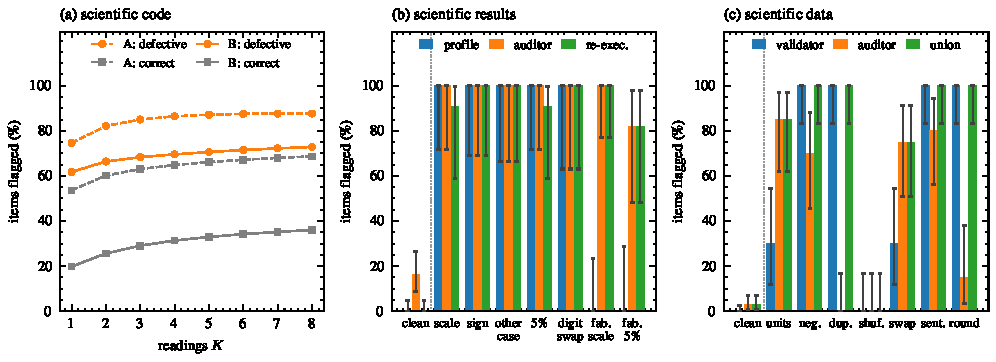
\includegraphics[width=\textwidth]{fig4_ai4s}
  \caption{\textbf{What each tier flags.} (a) Scientific code: the shipped auditor's union flag rate against
  the number of readings, on defective (orange) and correct (grey) instances, in arm A, whose task gave
  the whole problem (dashed), and arm B, whose task was reframed around the step (solid). (b) Scientific
  results and (c) scientific data, by fault type, with clean items leftmost: the deterministic tier
  (blue: the \texttt{science} profile in b, the documentation-derived validator in c), the model auditor at four
  readings (orange), and re-execution (b) or the union of the two (c) in green. In (c): mixed units,
  negated values, duplicated rows, shuffled target, swapped columns, $-999$ sentinel, rounding. The model auditor's flag is any
  model BLOCKER in the union of readings; the profile's is a hard failure, the validator's any fired
  check, re-execution's a value outside \texttt{np.allclose} defaults. Bars carry exact binomial 95\%
  intervals on the item counts (supplementary; they ignore clustering).}
  \label{fig:ai4s}
\end{figure*}

\subsection{Scientific code}
\label{sec:ai4s-code}

\textbf{Design.} SciCode \citep{tian2024scicode} decomposes research problems from 16 subfields into
steps with numeric tests written by scientists. The same frozen generator wrote every step three
times, each sample building on its own earlier steps. An instance is correct if it passes the step's
tests and defective if not; a step enters only if some sample passes it, which excluded 184 of 336 evaluated steps. This gives 81 defective instances (30 problems) and 150 correct ones (53 problems). Labels are per step, but the auditor sees the whole chain, and 51 of the defective and 49 of the correct instances have a failing earlier step (post hoc description). SciCode has no visible/hidden split, so
the auditor sees the step's prose, background, header and code, and no tests. The shipped
cross-vendor auditor and the generator's own model each read every instance eight times. After the
registered arm's outcomes, a second registered arm changed only the task text, naming the step's
function as the deliverable instead of opening with the whole problem; the program bytes are
identical (Appendix~\ref{sec:ai4s-code-full}).

\textbf{Results.} What the task named as the deliverable changed the flag rate substantially
(Figure~\ref{fig:ai4s}a). With the whole problem as the task, the shipped auditor
flagged 87.7\% [72.7, 98.6] of defective and 68.7\% [56.6, 79.7] of correct instances at eight
readings, and some of its objections to correct code were that one step did not implement the whole
problem. With the task reframed around the step, flags on correct code fell to 36.0\% [26.4, 45.6],
a paired change of $-32.7$ points [$-42.8$, $-22.4$]. Recall fell too, to 72.8\% [59.3, 87.3], a
change of $-14.8$ points [$-28.6$, $-2.7$], though the cluster sign-flip test for it gives
$p = 0.0625$. The change is the whole reframing (the step named, the problem description moved last
and marked as context, earlier functions exempted), and the arms ran in sequence. The generator's
own model's union recall was 46.9 points lower than the shipped auditor's in each arm ([$-63.0$, $-30.7$] and
[$-61.5$, $-34.4$]; a route comparison), while flagging 27.3\% [18.4, 37.3] and 18.0\% [11.5, 25.6]
of correct code, respectively.

At one reading in the reframed arm, the shipped auditor flags 61.7\% [47.9, 75.9] of defective and
19.8\% [12.9, 27.2] of correct instances: it discriminates, modestly. We read a seeded sample of 20 flagged correct instances whose earlier steps all pass, taking the first BLOCKER of the first flagged reading of each; four of the twenty concern earlier functions that the reframed task excluded from the deliverable. They range from real divergences between code and step text, through
contradictions inside the benchmark's own instructions, to tests too weak to separate outputs;
which flags point at defects was not established. An independent expert audit of SciCode found
self-contradictory specifications, non-reproducible gold answers and over-tight tolerances that
reject correct solutions \citep{hu2026scicodeverified}, so some instances labelled defective here
may be correct code the benchmark rejects. Of the 81 defective instances, 7 and 19 escaped all
sixteen readings of the two families in the two arms. Both raters judged 4 of 7 (two problems; cluster interval [0.0, 80.0]; $\kappa = -0.235$) and 13 of 19 (eight problems; [28.6, 93.5]; $\kappa = 0.587$) undetermined by the prose, too few problems and too little agreement for a stable share. The registered test that this share exceeds the general-code residual's 77.2\% is killed in both arms by its own interval rule.

\subsection{Scientific results}
\label{sec:ai4s-results}

\textbf{Design.} Each of 74 correct SciCode instances (36 problems) whose output on one seeded test
case is a real scalar or a short real array becomes a results increment: the program, the test's
inputs, a script that runs one on the other and writes a run log, a \texttt{results.json} citing each
value's log line, and a report whose numbers carry the product's number$\to$source annotations. Each
yields a clean item and a faulty one. Five fault types are \emph{reporting} faults, where the
artefacts disagree with each other or with the log; two are \emph{fabrications}, a $\times10^3$ slip
or a 5\% error written consistently into log, results and report. The model auditor reads each item
four times with the shipped \texttt{science} profile on; the profile's own verdict comes from the
same call; and re-execution compares the output with the report (Appendix~\ref{sec:ai4s-results-full}).

\textbf{Results.} The deterministic profile flags all 49 reporting faults and none of the 25
fabrications, because in those everything agrees with everything else (Figure~\ref{fig:ai4s}b). The
model auditor flags 23 of the 25 fabrications, 21 with a sound finding about the fault (post hoc),
usually by working the result out from the code, for example evaluating a KL divergence to 1 where
the report says 1000; the other two rest on wrong calculations. All 23 discordant items go the model's
way (exact McNemar $p = 2.4\times10^{-7}$). On reporting faults its rate is of the combined workflow,
since its prompt carried the profile's findings. Re-execution misses four faults whose change
to a near-zero output falls within \texttt{np.allclose}'s default absolute tolerance. Setting those four aside (post hoc), re-execution flags 70 of 70 faulty items at 0 of 70 clean, against the model auditor's 68 of 70 at 12 of 70. On the registered population the two flag 70 and 72 of 74 faulty items, and eight of the model's twelve clean-item flags identify real construction defects, so this subset favours re-execution for injected numerical faults without making it the better check in general. The model auditor also flags 12 of 74 clean items. Read one by one (post hoc),
8 correctly identify defects in our construction (a provenance sentence false where the benchmark
passes inputs as call literals; a unit label contradicting documented units); 4 rest on wrong
calculations or a syntax error that is not there.

\subsection{Scientific data}
\label{sec:ai4s-data}

\textbf{Design.} Four CC BY 4.0 physical-science tables \citep{yeh1998concrete, brooks1989airfoil,
tufekci2014ccpp, hamidieh2018superconductor}; 280 items of 120 rows with a data card giving each
column's meaning and unit: 140 clean, and 140 carrying one of seven faults (mixed units, negated
values, duplicated rows, a shuffled target, swapped columns, a $-999$ sentinel, rounding). Both model
families read each item four times, against a documentation-derived validator written from the card and
frozen before any item existed (Appendix~\ref{sec:ai4s-data-full}).

\textbf{Results.} The two tiers flag overlapping but different faulty items (Figure~\ref{fig:ai4s}c). The validator flags
92 of 140 faulty items (65.7\% [57.9, 73.6]) and no clean item; the shipped auditor 65 of 140 (46.4\%
[38.6, 54.3]) at 4 of 140 clean items (2.9\% [0.7, 5.7]); their union 112 (80.0\% [73.6, 86.4]) at the
same 4. These intervals resample items within dataset; four datasets are too few to resample, so no
interval carries between-dataset variation. The auditor's 4 clean flags and 4 of its faulty-item flags
are requests for fuller column descriptions on one card; counting only findings about the injected
fault (post hoc), the auditor flags 61 and the union 110.
Of the 20 faulty items the auditor flags and the validator misses, 18 carry a finding about the
injected fault itself (post hoc), mixed units or swapped columns; in one it argued that three atoms
spanning a 135\,pm radius range cannot have a mean radius of 1.6\,pm, the injected cell being that value converted to {\aa}ngstr\"oms.
It flagged no shuffled target and no duplicated rows (0 of 20 each), and did worse than the
validator on every fault the validator was written for. The generator's own model flags 67 of 140
clean items, and for at least 48 of those (a post hoc lower bound) one finding states a row count, field count, missing
column or truncation the file contradicts. The validator omits one range the concrete documentation
states and uses a list of continuous columns the card does not give.

\textbf{Held-out naming of faults at a fixed budget.} The counts above rest on flags, and their
diagnosis counts are post hoc. A further preregistered study asked, on 280 new items built the same way, whether the model auditor names faults the validator misses at a clean-flag budget fixed in advance. The endpoint was scored by code, not by a model: a flagging finding counts when it names the injected column (both columns
for a swap; duplication for duplicated rows), read from the injection manifest. The rule is lexical and is not a measure of correct diagnosis. Operating points were fixed on the items above: the smallest vote threshold over four readings with a clean-flag rate of at most 10\% (one reading for the shipped auditor, all four for the generator's own model). On the held-out items the validator meets the rule on 90 of 140 faulty items
(64.3\% [56.4, 72.1]) at no clean flag, and the validator with the shipped auditor 105 (75.0\%
[67.6, 81.9]) at 9 of 140 clean flags (6.4\% [2.8, 10.5]): $+10.7$ points [6.0, 15.9], 15 items one
way and none the other (exact McNemar $p = 6.1\times10^{-5}$), the registered primary. At its own operating point the generator's own model meets it on 40 at 14 clean flags, 12.1 points [4.1, 20.3] fewer than the shipped auditor (a route comparison). The rule also counts some findings about other things. On the study agent's unblinded post hoc reading of the 15 items the union adds, 14 locate the fault in the right columns ($+10.0$ points [5.4, 15.1]) and 11 also explain it ($+7.9$ [3.7, 12.5]; Appendix~\ref{sec:ai4s-data-full}).

\section{Method in full}
\label{sec:method}

\subsection{Substrate, population and ground truth}

Every result in this paper is measured on one substrate: HumanEval+ and MBPP+ (EvalPlus),
Python functions whose median task is 41 words of prose and 6 lines of reference code, each with
an executable hidden test suite. Every stratum, recall denominator and false-positive population
is therefore decided by an interpreter, and no model judges a recall or false-positive outcome.
The one outcome defined by adjudication, correct diagnosis in the clarification study, is judged
jointly by two models and is labelled so where it appears. The benchmark's base suite is shown to
the generator as the \emph{visible} suite, and its plus suite is held back as the \emph{hidden}
one. A second substrate, the standard-library half of BigCodeBench, was built and audited and
closed without a quotable number when its preregistered criterion was not met on a third run;
nothing from it is reported here.

\textbf{How the population was built.} The corpus has 542 problems. Two, \texttt{HumanEval/32}
and \texttt{Mbpp/590}, were excluded by name before generation because their own reference
solutions fail their own hidden suites in this harness, which leaves 540. One frozen generator,
\texttt{claude-haiku-4-5-20251001}, was shown each specification and its visible suite and wrote
one solution per problem. A candidate that passes the visible suite and fails the hidden one is a
\emph{defective} instance; one that passes both we call \emph{correct}; one that fails the visible
suite is discarded from every recall and false-positive population. The defect stratum is small,
about 10\% of solutions, so under a rule registered before the second pass and depending only on
execution outcomes, generation was repeated over the same 540 problems until there were at least
100 defective instances or three passes. It stopped at two: 56 and 54 defective, 455 and 455
correct, 29 and 31 discarded. An instance is therefore a (pass, problem) pair, and one problem can
contribute two. Recall is measured on all \textbf{110} defective instances, which come from
\textbf{56 problems}; false positives on \textbf{150} of the 910 correct instances, drawn once
from a fixed seed before any auditor ran, from 143 problems. Seven of the 110 defective instances
fail by not terminating rather than by a failed assertion, and the registered population keeps
them.

Two consequences of these definitions hold throughout. \emph{Correct} means \emph{passes the
hidden suite}. It is a benchmark label produced by an interpreter, not a guarantee that the
program meets its specification, and a suite can be incomplete or wrong. Since this paper's own
third result is that a specification often fails to determine what the hidden suite asks, we
cannot treat passing that suite as correctness in the ordinary sense, and a \emph{false positive}
is likewise a flag on test-passing code rather than a demonstrated mistake by the auditor. And the
defect population is not a sample of model-written code: it is the residue that already survived
the visible tests, which is by construction the harder part. A recall figure here is the fraction
of that residue an auditor catches, never the fraction of all defects a model writes.

\subsection{The auditor and the estimand}

The auditor reads the specification, the visible tests and the candidate, and returns findings
with severities; an increment is blocked when any finding is graded BLOCKER. It never sees the
hidden suite. The estimand throughout is \textbf{union recall at $K$}: the fraction of defective
instances blocked by at least one of $K$ independent readings, averaged exactly over all
$\binom{K_{\max}}{K}$ subsets rather than by sampling. The matching quantity on the correct stratum
is the union false-positive rate, and a union recall figure is reported only beside the
false-positive rate it cost.

Four auditor routes appear below. The shipped cross-vendor auditor is \texttt{gpt-5.6-terra}; the
same-vendor auditor is \texttt{claude-haiku-4-5}, the generator's own family and size; the
stronger same-vendor auditor is \texttt{claude-sonnet-4.6}; and a third family,
\texttt{gpt-6-astra} at high reasoning, is read at $K=4$. The auditor's constitution, its prompt
builder and every route's capability card are in the auditor harness, a separate repository, at
the commit named in the provenance file, whose per-reading records carry the hash of every prompt
actually sent.

The routes are \textbf{not sampled alike}, and this bounds every cross-family union-of-$K$
contrast in the paper. The cross-vendor route's capability card does not permit a sampling
temperature, so no sampling parameter is sent and the route varies between readings. The
same-vendor routes permit one, and the layer sends temperature $0$, so those routes are nearly
deterministic. A union over readings that do not differ cannot grow, so the two families' unions
are not equally free to rise with $K$, and a cross-family difference in union recall confounds
auditing ability with how much each union could grow. The asymmetry is a property of the shipped
routing layer we measured rather than a design choice. We did not discover it until after the
runs, and we report the $K=1$ contrast beside the $K=8$ contrast wherever it matters. A
temperature-matched replication is the first item in \S\ref{sec:limits}.

\subsection{Statistics}
\label{sec:stats}

The unit of observation is the instance and the resampling unit is the problem, because problems
recur across generation batches and instances sharing a problem are not independent. The $K$
readings of an instance are repeated measurements of it, not $K$ further independent
observations. The bootstrap over problems estimates uncertainty from which tasks the benchmark
happens to contain. It does not estimate how much a fresh batch of model calls on the same tasks
would move the numbers, which would need replicate runs we did not budget for at every arm.

Every rate carries a 95\% percentile bootstrap over whole problem clusters (10{,}000 resamples,
seeds fixed in each preregistration), with the Wilson interval printed beside it and marked as too
narrow. Paired contrasts carry an exact McNemar test and a cluster-level sign-flip permutation
test. Where every discordant pair points one way, the percentile bootstrap's bound at zero is an
artefact, and an unconditional interval (grid-approximated, unclustered) is quoted instead. The
one exception is the clarification study, whose registration fixed the bootstrap for a contrast
that turned out one-signed; its interval is reported as registered and read beside its exact
cluster test (\S\ref{sec:inreview}). A saturation curve is summarised by a constrained
exponential fit, and the fitted asymptote is quoted only when the preregistered flattening bar is
met; otherwise it is labelled an extrapolation and the raw union at $K_{\max}$ is the number
quoted. Counts of five or fewer are quoted as counts. Multiplicity is handled per study as each
registered it: the study carrying the primary contrasts corrects over every comparison it
computed, a Bonferroni family of sixteen with a threshold of $0.00313$ that two comparisons clear;
others registered a single primary, and study 19 reports its twenty further quantities without
correction.

We measured interval coverage by simulation rather than assuming it. Under the two strata's
actual cluster profiles (110 instances in 56 problems, and 150 in 143), with within-problem
concordance $0.5$, the percentile bootstrap's coverage of a nominal $95\%$ rate interval is as
follows, over 400 replicates of 600 resamples each. The Monte Carlo standard error is about 0.011
near 95\% coverage and 0.020 at the lowest cell; the simulation covers single rates only, and uses
integer-index percentiles where the analyses interpolate (\texttt{analysis/coverage\_simulation.py}).

\begin{center}\small
\footnotesize\setlength{\tabcolsep}{2.5pt}
\begin{tabular}{@{}lccccccc@{}}
\toprule
true rate & 0.03 & 0.05 & 0.10 & 0.16 & 0.30 & 0.48 & 0.60 \\
\midrule
defect (56) & 0.798 & 0.870 & 0.933 & 0.933 & 0.953 & 0.935 & 0.928 \\
correct (143) & 0.888 & 0.918 & 0.938 & 0.933 & 0.943 & 0.955 & 0.965 \\
\bottomrule
\end{tabular}
\end{center}

\noindent In these simulations coverage is near nominal at the true rates this paper's headlines
sit at and \textbf{badly anticonservative at small true rates}: at a true rate of $0.03$ on the
defect stratum the simulated interval covers about $0.80$, not $0.95$. This is evidence of
potential undercoverage for analogous intervals, not a measured coverage of any interval quoted
here. Intervals on rates below roughly $0.10$ may be narrower than they claim. The simulation
costs no model calls. Two earlier paired-contrast constructions in this programme were found by
review to cover $0.416$ and $0.075$ where $0.95$ was claimed, and both were replaced. No sample
size was justified in advance by a minimum-detectable-effect calculation.

\textbf{An interval that contains zero is reported as one that does not exclude zero, and nothing
more.} No equivalence margin was registered anywhere in this programme and no equivalence test was
performed, so none of those intervals is evidence that two conditions are alike or that an
intervention did nothing. This work once inferred equal cost from an interval containing zero and
withdrew the inference on review. Where a hypothesis fails its registered criterion we say it
failed, not that the effect is absent.

All analysis is plain Python 3.13 using only the standard library (\texttt{random},
\texttt{math}, \texttt{itertools}, \texttt{csv} and \texttt{json}). The bootstrap, the exact
McNemar test, the cluster sign-flip permutation and the exact subset enumeration behind every
union-at-$K$ figure are implemented in the repository rather than called from a numerical package,
so each can be read where it is used and none depends on a third-party version.

\subsection{Preregistration and independent review}
\label{sec:methods-review}

\textbf{Who did what.} The studies were designed, run, analysed and written up by an AI research
agent, Claude (Anthropic; \texttt{claude-opus-5} and \texttt{claude-fable-5-1}, working in Claude
Code), under the direction of the author, who is responsible for the work. Wherever a rating or
adjudication below is attributed to \texttt{L1}, the rater was that agent. It wrote the rubrics,
knew the hypotheses and the earlier labels, and is from the same vendor as the generator.
\textbf{No human rated or adjudicated anything in this paper.} Every report was then reviewed by a
second model, \texttt{gpt-6-astra}, as described below.

Each study that made model calls was preregistered before its first one, fixing its population,
hypotheses, primary outcome, intervals, kill conditions, budget and stopping rule, with two
exceptions. First, the severity sweep of \S\ref{sec:auditor} re-grades findings already archived,
makes no model calls, and was never registered: every figure it produces is post hoc and
exploratory, and none is a confirmatory test. Second, the analysis behind
\S\ref{sec:inreview}'s third-rating result was registered a day \emph{after} its contrast had been
computed and committed, in a document that claimed the opposite; that document is withdrawn in
the repository and the analysis is registered nowhere. Its method was fixed in advance by an
earlier amendment, but the disjoint reading, the abstention-excluded secondary and the
broken-sheet comparison were not.

Planned departures are numbered amendments committed before the step they govern, each recording
what was known at the time. Deviations discovered only afterwards, such as a leak check or a spend
guard implemented more narrowly than registered, are disclosed in the report and are not
amendments. Where an amendment followed an interim observation, the results say so and argue
whether the change could favour the hypothesis.

Each report was then reviewed by a model from a different vendor to the generator, with read
access to the raw records, asked to re-run the analysis, recompute the intervals independently,
and check every sentence against the records. \textbf{That reviewer is \texttt{gpt-6-astra}},
which is also one of the auditor families measured in \S\ref{sec:auditor}, one of the two raters
behind \S\ref{sec:residual}'s labels, and one of the two adjudicators whose joint labels define
the clarification study's outcome. For most claims this is a cross-vendor check on work the
reviewer had no part in. For the claims that rank \texttt{astra} against the other families, and
for the clarification study's adjudication, the reviewer is the subject, and those results should
be read as self-assessed until a model that audited nothing in this programme has checked them.
This project's own P3 Amendment 10 disqualified the same model as the clarification study's
manipulation-check rater for the same reason, yet kept it as that study's second adjudicator and
its reviewer; the standard was applied unevenly within one study, and not applied to the review
at all until a pre-submission referee pointed it out.

Reviews are archived verbatim, including those that refused approval, and several studies needed
many rounds. On one day five reports were refused at once, and clearing those five took
thirty-one further rounds. In most of them what moved was what the reports claimed about their
measurements, and in most of the later refusals the object was a repair written to satisfy the
previous round rather than the study it repaired. A fix written to satisfy a reviewer is itself an
unreviewed claim; that is the most transferable thing this process taught us.

\textbf{The reviewer is a language model, and this paper is about the ceiling on language models
reading code they did not write.} That applies to our own instrument. The studies of
\S\ref{sec:inreview} cleared review at rounds \textbf{3, 3, 4, 6, 7, 9, 10 and 11}, and the
ceiling study behind the headlines at 21; in every case the round before the last still returned
substantive findings. Some of those findings were defects introduced by the repairs between
rounds, so the counts do not estimate a single pass's recall; they show only that no report
cleared in fewer than three. \emph{Quotable at round $N$} means a report survived $N$ passes, not
that it was verified, and the marks in this paper should be read as a filter of unknown recall.

Two further points follow. First, measurements did move on review. The severity sweep's first
review found its loader misreading one family's draws and another's population, and every
cross-family figure was recomputed; the clarification study's second review moved its primary
from 9 of 31 to 9 of 32 instances and its contrast from $+29.0$ to $+28.1$ points, by finding an
instance wrongly excluded; and a label count inside a reviewed report was 71 where its data say
67. Once a figure's inputs were right, the reviewers reproduced rates, intervals, subset
enumerations and seeds independently and found no arithmetic error, and most refusals were about
what the prose claimed. On recomputation the instrument is strong; on interpretation it is weak,
and the two should not be quoted as one assurance. Second, the class of defect this leaves open is
the one that looks right to a language model. The clarification study audited the wrong program
for 384 readings, because a per-problem field was used where a per-instance one was needed, and
every automated gate passed: each checked that the code was \emph{identical across conditions},
and it was, identically wrong. The agent found it while reading an adjudication sheet, by noticing
that a displayed program returned exactly what its hidden suite was said to reject. Neither the
gates nor a reviewer found it, and we do not know what else of that kind remains.

\textbf{Every review prompt in this programme stated the claimed result before the reviewer
began.} We tried to test what that costs, and the attempt failed. One report, quotable at round 6
after five refusals and unchanged since, was dispatched again under a prompt whose own text
withheld every figure and every prior verdict and asked for an independent computation first.
That prompt's list of binding artefacts then named two files that state those figures, one of
them the claims-ledger entry for the result under review. The blinding was not enforced, so the
agreement between that pass and the briefed one establishes nothing. What the pass did return is a
disagreement count: six substantive findings that six briefed rounds on the same file had not
produced, among them that the report's two groups were two different definitions of
\emph{caught} rather than one population with duplicate rows, that its rating sheet displays at
most three failing inputs while 81 of its 121 entries have more recorded, and that a count of
changed labels was 71 where the data say 67. \textbf{That count is $n=1$, uncontrolled and
unregistered.} A seventh round might have found new things under any prompt, and no matched
briefed round was run against the same file. We report it as a reason to test blinding properly
rather than as a result about blinding. Later first rounds withheld the conclusions from the
prompt text, but the report under review stayed among the named artefacts, with an instruction to
derive the result before reading it; that is a request, not blinding.

Every study drawn on here has completed that review. One further study was re-run twice and closed
without a quotable number; the paper names it only to say what it no longer supports.

\section{Results on general-purpose code in full}
\label{sec:results}
The claims this paper defends, each with its interval and its label, are listed in
\texttt{CLAIMS.md}. A claim enters that file only after its report has passed an independent
review by a model from a different vendor with access to the raw records, and every section below
draws only on such reports. Section~\ref{sec:inreview} reports eight studies whose reviews took
between three and eleven rounds each to reach that point, and states what each does and does not
license. The headline results of \S\ref{sec:repeat}--\S\ref{sec:residual} come from the ceiling
study; where they cite a study from \S\ref{sec:inreview}, they say so.

Rates carry the 95\% problem-cluster percentile bootstrap as the primary interval. Problems recur
across generation batches, and an interval that treats instances as independent is too narrow.
Where the source report gives a Wilson interval, it appears beside the bootstrap. For single
rates, simulations of an analogous interval under this clustered design (\S\ref{sec:stats})
suggest coverage near nominal at the headlines' rates and possible undercoverage below a true rate
of about $0.10$, under an assumed within-problem correlation. They do not measure the coverage of
the intervals reported here, and the paired contrasts and category-conditioned shares have no
measured coverage.

Sixteen comparisons were computed in the study that carries the primary contrasts, under one
Bonferroni family with a threshold of $0.00313$. That correction is applied to $p$ values and
never to intervals. Every interval in this paper is an unadjusted 95\% interval, so a directed
statement resting on an interval alone, with no $p$ value that clears its family, is worded as a
direction rather than as a finding. Each $p$ value belongs to the family of the study that computed
it. Those in \S\ref{sec:rulebook} are members of that sixteen-member family. The one in
\S\ref{sec:auditor} is the auditor-family study's single registered primary, so there was no family
to correct within; it would also clear $0.00313$. The clarification study's $p$ values are reported
beside a primary registered on its interval, and no correction was registered for them. Where a $p$ value appears
below, the exact McNemar value and the cluster-level sign-flip permutation value are both given,
because instances within a problem are not independent and only the second respects that.


Table~\ref{tab:primary} (Section~\ref{sec:ceiling}) collects selected primary quantities with their populations and labels;
the prose gives each one where it is used.

\subsection{Returns to repeated reading diminish short of complete}
\label{sec:repeat}

The shipped cross-vendor auditor reads an increment holistically and returns findings; an
increment is blocked if any finding is graded BLOCKER. Over eight independent readings of the same
110 defective instances, union recall rises from 10.7\% at one reading to 30.0\% [20.0, 40.7] at
eight (Figure~\ref{fig:saturation}). The eighth reading still adds 1.93 points, cluster [1.14,
2.78], against the flattening bar of 1.0 points registered before the first model call, so the bar
was not met. Under exact subset averaging that statistic has a closed form: the number of
instances flagged by exactly one of the $K$ readings divided by $K n$, here $17/(8\cdot110)$. It
is a count of singletons, not a fitted slope. Its interval resamples problems and so carries
task-sampling variance. The statistic itself is made of reading-sampling variance, which the
interval does not describe. The bar should therefore be read as a statement about these 17
instances, not about a population slope.

The constrained fit puts the asymptote at 31.5\%, but on our own registered criterion that figure
is an extrapolation, and the raw union at eight readings is the number to quote. What the data
support is diminishing returns at the budget we could afford, not saturation: at 1.9 points per
reading the curve was still climbing when we stopped. The bar also depends on where a family was
stopped. Exact subset-averaged increments do not grow with $K$ (this curve's is 2.9 points at the
fourth reading and 1.9 at the eighth), so a fixed bar is harder to meet at $K = 4$ than at
$K = 8$, and meeting it at either says little by itself about where the curve ends.

Twenty readings pooled across three auditor families reach 48.2\% [36.7, 60.0], and the same
twenty readings flag 54 of 150 correct increments, 36.0\% [28.2, 44.2]. That is more than
twice the shipped route's 16.0\%, so pooling buys its coverage at its own price. Those twenty
readings are also not twenty opportunities. The pool is eight cross-vendor, eight same-vendor and
four \texttt{astra} readings, and the same-vendor route gains 1.8 points from its first reading to
its eighth against the cross-vendor route's 19.3. It is sent temperature $0$ and returns nearly the
same verdict each time, though this design cannot say how much of that is the temperature and how
much the model. Counting that route as roughly one reading puts the depth nearer thirteen than
twenty (a heuristic, not an estimate), and the pooled figure should be read as a union over three
routes rather than over twenty independent looks.

The price is measured on the same footing. Union false positives on 150 correct increments reach
16.0\% [10.1, 22.3] at eight readings. We also compute the recall bought per point of false
positive: recall gained over one reading divided by false positives gained over one reading. It is
1.68 at eight readings and changes little as readings accumulate. From $K=2$ to $K=8$ the
ratio runs 1.67, 1.63, 1.64, 1.65, 1.66, 1.67, 1.68. It falls once, at $K=3$, and then rises, so repeated
reading on this route buys recall at a slightly improving price. The ratio is a quotient of two
measured rates and carries no interval of its own.



\subsection{Which model reads, and under which severity rule}
\label{sec:auditor}

Replacing the auditor with a stronger model of the generator's own vendor moved union recall at
eight readings by $-26.4$ points, cluster $[-37.3, -15.6]$: 4 of 110 against 33 of 110. Three
instances were flagged only by the new family and thirty-two only by the shipped auditor, at an
exact McNemar $p$ of $4.2 \times 10^{-7}$ and a cluster sign-flip $p$ of $2.0 \times 10^{-5}$.
This was the auditor-family study's single preregistered primary, so no family correction applies. Three
measurements qualify what it means, and none of them favours reading it as a statement about
auditing ability.

First, the two auditors are not at the same operating point, and this paper elsewhere warns against
comparing auditors at different operating points. The stronger model flags correct code at
3.3\%, or 5 of 150, which \S\ref{sec:stats} says to quote as a count. Its bootstrap interval,
[0.7, 6.7], sits in the range where simulations of an analogous interval cover about $0.89$ at a true rate of $0.03$
rather than $0.95$, so it may be narrower than it claims. The shipped auditor flags 16.0\% [10.1,
22.3]. The stronger model blocks less of everything.

Second, the sign reverses under a weaker severity rule (Figure~\ref{fig:sweep}). That rule counts
any finding rather than only findings graded BLOCKER; it is exploratory and was not
preregistered. Under it the stronger model reaches 59.1\% [47.3, 70.6] on the defect population at
34.0\% [26.5, 41.7] on correct code, and the shipped auditor reaches 34.5\% [23.6, 45.5] at
19.3\% [12.8, 26.3]. The ratio of recall to false positives, a derived point ratio with no
interval, is 1.74 for the stronger model and 1.79 for the shipped auditor, so nothing here shows
one family buying more recall per false positive than the other. Under
any-finding grading the stronger model's findings cover more instances, and under the BLOCKER rule
fewer, so the $-26.4$ depends on the counting rule. That does not show why the families' findings
differ, or that any finding identifies the hidden failure.

Third, the two families are not sampled alike. The shipped cross-vendor route's capability card
does not permit a temperature, so no sampling parameter is sent and the route varies between
readings; the same-vendor route permits one, the layer sends temperature $0$, and that route is
nearly deterministic. A union over nearly identical readings cannot grow much, and it does not:
over $K = 1$ to $8$ the cross-vendor family gains 19.3 points and the stronger same-vendor family gains
3.0. At one reading the gap between them is $-10.1$ points, not $-26.4$. The rest accumulates as
the two unions grow at different rates, and because model and sampling differ together, the
design cannot say how much of that difference is the sampling and how much the model. We regard
this as the most serious limitation of the contrast, and \S\ref{sec:limits} records what would be
needed to remove it.

A third family points the other way and belongs beside the headline. A high-reasoning model of the
cross-vendor family reaches 32.7\% [20.7, 45.0] union recall at four readings while flagging
10.7\% [5.9, 16.1] of correct code, against the shipped auditor's 30.0\% at 16.0\% with eight.
Paired on the same instances, the two advantages are never established together. At a common four
readings it leads on recall, $+11.5$ [2.9, 21.3], with an unresolved false-positive difference
of $-0.3$ $[-3.8, +3.4]$; against the shipped auditor's full eight it leads on false positives,
$-5.3$ $[-10.3, -0.7]$ unadjusted, but not on recall, $+2.7$ $[-6.5, +13.0]$
(\S\ref{sec:inreview}). The evidence therefore does not support ``a stronger model is a worse
auditor''. It supports the narrower statement that this particular same-vendor model, under the
preregistered BLOCKER rule and sampled at temperature $0$, blocks far less.

A same-vendor route of the generator's own size reached lower union recall than the
cross-vendor one on these instances, $-12.7$ points $[-25.0, -0.9]$ at eight readings, signed so
that a negative value favours the cross-vendor route. The interval is unadjusted, its upper end is
0.9 points from zero, and that route is sent temperature $0$, so this is a direction under this
sampling and not a ranking of auditors. A study on a second substrate was meant to test whether the
sign reverses there; it closed without a quotable number, and on its clean run the same contrast
included zero, so no reversal was established either (\S\ref{sec:inreview}). The figure above is
a measurement on this substrate, and whether it is a property of same-vendor auditing is open.


\begin{figure}[t]
\centering
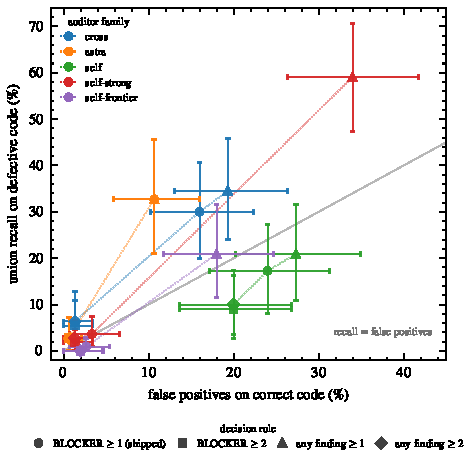
\includegraphics[width=0.46\textwidth]{fig2_sweep}
\caption{\textbf{Union recall is a property of the decision rule, not only of the auditor.}
Each point is one auditor family re-graded under one of four decision rules on the same archived
readings, with problem-cluster 95\% intervals on both axes; no new model calls were made. The
families are read at different depths: \texttt{cross}, \texttt{self} and \texttt{self-strong} at
all eight of their readings, \texttt{astra} and \texttt{self-frontier} at their four. The figure
therefore places each family at its full archived depth and is not an equal-depth comparison; the
common-depth contrasts are in Table~\ref{tab:primary}. The dotted guides join a family's four
points and are not a measured curve. Two things Table~\ref{tab:primary} cannot show: the families
do not lie on one frontier, and \texttt{self-strong} has no point under the four deterministic
rules between 3.3\% and 34.0\% false positives, exactly where a comparison matched to the
cross-vendor auditor would sit, so its ranking there is bracketed rather than measured. Nothing in
this figure assesses finding content; a flag is not a diagnosis.}
\label{fig:sweep}
\end{figure}

\subsection{One rulebook sentence moves flags, and does not measurably move outcomes}
\label{sec:rulebook}

Adding a single rule to the auditor's constitution, telling it to find what the visible tests do
not cover, moved flags on the defect population from 10 of 56 to 25 of 56: $+26.8$ points, cluster
[13.6, 40.4], exact McNemar $p = 0.0003$, cluster sign-flip $p = 0.0009$. Together with the pooled
defect-and-correct flag contrast, this is one of only two comparisons that clear the Bonferroni
threshold, and the two are the same effect seen twice.

The estimand is narrower than that of the sections above and must be read at its own scale. It is measured
on 56 instances from 41 problems, not the 110-instance defect population. It is recall at a single
reading, union recall at $K = 1$ on that population, because every loop arm revises once. And it
is exploratory, because the preregistration named outcome contrasts rather than flag contrasts. For
those reasons we do not compare its magnitude with the $-26.4$ or the $+19.3$ of the preceding
sections, which are union-recall differences at $K=8$ over 110 instances (a contrast between
routes and a gain from $K=1$).

Two costs travel with it. On correct code the same rule moved flags by $+12.50$ points. Every
discordant pair points the same way (7 against 0), so by the rule stated in \S\ref{sec:stats} the
percentile bootstrap's bound at zero is an artefact, and the admissible interval is the
unconditional one. That interval is $[-3.6, +26.8]$ and does not exclude zero. It is approximate
rather than guaranteed exact, because it uses a grid-approximated nuisance supremum and ignores
clustering. Its exact McNemar and cluster sign-flip $p$ are both $0.0156$, against that study's
Bonferroni threshold of $0.00313$. The directed statement the records
support is the pooled one, where 23 discordant pairs point one way and 1 the other (exact McNemar
$p = 3.0\times10^{-6}$, cluster sign-flip $p = 1.0\times10^{-5}$): the sentence makes the auditor
louder overall. On the correct stratum alone the cost is $+12.50$ points with an interval that
contains zero.

The second cost is to outcomes. The contrast that isolates the rule compares the arm with the
added rule against the cross-vendor arm on hidden-suite pass rate after one revision, over both
strata (112 instances on 96 problems). The effect is $+5.36$ points, cluster $[-0.89, +12.07]$,
exact McNemar $p = 0.146$ and cluster sign-flip $p = 0.183$; the interval does not exclude zero. The rule demonstrably moves what
the auditor writes down. Whether that converts into code that passes the hidden suite is not
established, and since this paper argues that a flag is not a catch, that distinction applies to
our own intervention first.


\subsection{Most of what the auditor missed is failure the specification never determined}
\label{sec:residual}

Fifty-seven of the 110 defective instances were flagged by no reading of the three families read
at that point. That is a statement about twenty readings, not about detectability. If an instance
is caught with probability $p$ on each independent reading, twenty readings miss it with
probability $(1-p)^{20}$, which is still $98\%$ at $p = 0.001$ and $36\%$ at $p = 0.05$. Never
flagged here does not mean never flaggable, and we use the residual as a population to
characterise rather than as a set of defects shown to be invisible.

We can put a number on how flaggable it is. Reading six families at forty readings, including the
same auditor under a rulebook with one sentence added, shrinks the never-flagged set from 57 to
32 of 110, and 43 of the 68 instances both raters call specification-undetermined
are flagged by some reading of some family. Being undetermined is not sufficient for being
missed. What does not move is the composition: the undetermined share of the never-flagged set is
44 of 57, $77.2\%$, at three families and twenty readings, and 25 of 32,
$78.1\%$, at six families and forty readings.

The first classification of that residual asked whether the visible tests exercised the failing
input before it asked anything else, and it called 46 of 57 unexercised edges. Re-rating the same
instances under a second protocol reverses that. The second protocol asks first whether the
specification's prose determines the hidden suite's expected value, redefines the categories by
entailment, and uses two raters in consensus; ordering, definitions and raters all changed
together, and the study cannot isolate which mattered. The two raters agree that 44 of 57
(77.2\%, cluster [62.1, 91.1]) are cases where the prose does not settle the value, and that 2 of
57 are cases where it does and the visible tests merely never built the input. The preregistered
condition for withdrawing ``the residual is mostly unexercised edge'' fires on both of its
clauses, and that claim is withdrawn. The interval is conditional on a category and has no
committed coverage simulation, so it is uncalibrated, as is every category-conditioned interval we
report.

A classification that reverses when its protocol changes is, by itself, weak evidence about the
auditor, and the raters are not independent of it: one was the agent that ran this programme
(\S\ref{sec:methods-review}), which wrote the rubric and knew the earlier labels and which claim
was at stake. Three things support the second reading. The rubric was fixed before any label was
written. The labels were committed before we looked for outside evidence. And when a first pass
was found to have carried instance identifiers and a sheet name into the raters' view, the
labelling was re-run with identities stripped and the result held. An outside party had also
independently recorded specifications as defective, in twelve MBPP tasks named in a paper written
for another purpose \citep{richter2026collapse}. Of the 11 that fall inside our
defect population, our raters agree on 9, and both disagreements lie on the boundary that paper's
own ``incomplete'' category draws. That check is one-sided by construction: it can support agreement where an
outsider looked, and can bound nothing about the rate.

\textbf{A rater outside the residual's families, asked a different question.} One of the two
raters above is \texttt{gpt-6-astra}, whose own misses help define the residual. A model that is
not one of the families defining it, \texttt{gpt-5.6-luna} (which read these instances only as a
secondary audit route in an earlier architecture study), later rated the same 57 instances post
hoc under a different rubric: whether the prose determines an answer at all, on a sheet showing at
most three failing inputs and never the expected values (\S\ref{sec:inreview}). It labels
38 of 57 undetermined, 13 determined and 6 cannot-tell. The two figures measure different
constructs. The earlier category also admits prose that determines an answer the oracle
contradicts, which this rubric does not count as undetermined, so 38 is not a corrected estimate
of 44. What they share is that a participating and a non-participating rater both put a majority
of the residual on the undetermined side. The non-participating rater agreed with itself on only
7 of 11 repeated items.


\begin{figure*}[t]
\centering
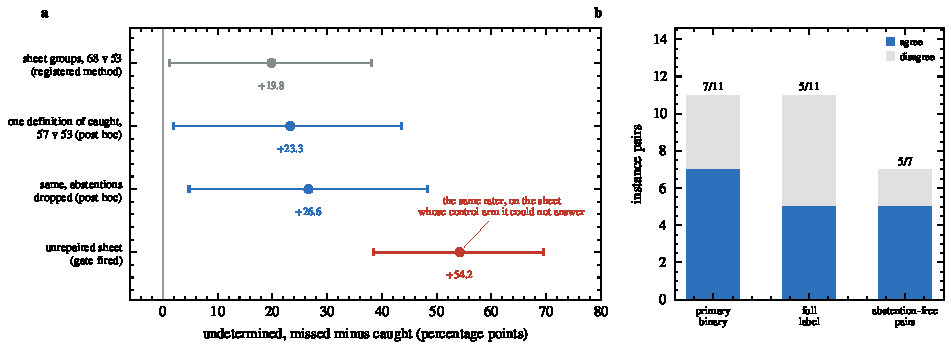
\includegraphics[width=0.94\textwidth]{fig3_residual}
\caption{\textbf{The residual contrast, printed beside the instrument that produced it.}
a, The share of instances a rater judged specification-undetermined, missed group minus
caught group, under each reading, with problem-cluster 95\% intervals. The two sheet groups use
different definitions of \emph{caught} and share eleven instances, so the two readings that apply
one definition are the ones that compare populations; both are post hoc. The red point is the same
rater on the same sheet before its control arm was rebuilt, when 42 of 53 caught entries carried
no failing-input evidence and all 42 drew \texttt{cannot-tell}. With that arm the contrast was
larger and pointed the way the hypothesis points. The repair and a fresh model run changed
together, so presentation, sampling and batch context are not separated, and a preregistered
one-third \texttt{cannot-tell} gate excluded the earlier figure. b, The same rater's agreement with itself on
the eleven instances the sheet carries twice, with identical text and identical evidence. The
contrast in a is read off the instrument in b, and the claim this paper draws
from it is stated under that constraint.}
\label{fig:residual}
\end{figure*}

\subsection{Nine further studies, and what they license}
\label{sec:inreview}

Eight further studies cleared independent review after between three and eleven rounds each, and a
ninth, on a second substrate, closed without a quotable number. We
report them here rather than folding them into the sections above because several are narrow or
negative results whose limits are part of the claim, and because the shape of their refusals is
itself a finding about this method.

\textbf{A rulebook sentence moves a second vendor's family.} The referent rule, \emph{find what the
visible tests do not cover}, raises union BLOCKER recall on \texttt{self-strong} (\texttt{claude-sonnet-4-6})
at four readings by +20.9 points, cluster [10.8, 31.8], at a false-positive cost on
correct code of +8.0 points [3.4, 12.7]. This reproduces \S\ref{sec:rulebook}'s effect on a different vendor's model at a
different $K$, with its own price. A second intervention, a rule on how findings are graded, shows
no demonstrated improvement: $+0.9$ points $[-1.8, +4.5]$. That hypothesis fails its registered
criterion, and the failure demonstrates neither equivalence nor that the rule did nothing. The
same study also measured, post hoc, whether a flagged finding \emph{reports a failure} on the
instance's failing input class, that is, says that class raises or returns the wrong value. The
count is 3 of 110 (2.7\% [0.0, 7.3]) under the shipped constitution and 27 of 110 (24.5\%
[14.4, 35.7]) under the referent rule (not the grading rule), and it may not be
quoted as defect recognition. Its rubric admits a finding even
where it grades the class non-blocking or says the specification is silent, so findings that
disclaim the requirement are counted in.

\textbf{The added rule raises union recall to 60.9\%; a higher ceiling is not established.}
On the defect population the referent rule takes union recall from 33 of 110 to 67 of 110, or 60.9\%
[48.6, 72.5]. This is the same quantity as the shipped auditor's eight-reading headline in
\S\ref{sec:repeat}: blocked by at least one BLOCKER, unioned over eight readings, here for the
shipped auditor with the referent rule against the shipped auditor alone. The gain is +30.9 points [19.1, 43.1], at a cost of +20.7 points
[12.8, 28.8] in false positives. The single-draw false-positive rate is 23.6\% [17.1, 30.3] and
fails the product bar on all eight draws. The caution that a flag is not a catch attaches to both figures equally. What separates
them is their price, 36.7\% [28.5, 44.8] false positives against 16.0\%, which is why the shipped
route is the shipped route. The fitted asymptotes differ by $+27.1$ points [10.9, 39.0], and
\emph{that does not establish a higher ceiling}. The cross-vendor arm never flattened, so one of
the two terms is an extrapolation. Heterogeneous low-probability detection imitates a ceiling at
this budget, since an instance found with probability $0.02$ per reading survives eight readings
about 85\% of the time. And this study's own zero-inflated estimator finds no never-detectable
class in \emph{either} arm. The study's adjudication kill is arithmetic rather than a labelling
artefact. Only 9 of 110 instances drew any finding on the single reading whose finding texts were
archived, so the largest defect-asserting count available under perfect adjudication was 9, below
the floor of 20. Every adjudication-derived figure in the study is conditional on labels whose
production can no longer be audited. One rater's raw reply, prompt, launcher and execution log
lived only in a session scratchpad, and they were destroyed between the review that flagged them
and the repair.

\textbf{Corroboration does not validate a generated test.} A wrong generated test, one that fails
on the dataset's canonical solution, is not reliably recognised by asking whether further
independent generation draws also fail on the same candidate. Neither rule that makes further generation calls reaches the
preregistered threshold on the registered population. That population covers failing
applications on all three candidate strata; 58 of its 107 failing applications are on candidates
that already fail their visible tests. The retained wrong-test rates are 12.2\% [3.6, 22.6]
(Wilson [7.0, 20.6]) for majority-over-draws and 14.9\% [6.5, 25.5] for any-draw agreement,
against a limit of 2\%. Neither is shown to improve on the free within-draw comparator at 12.8\%
[3.9, 23.9]: the better of the two rules keeps the same wrong applications plus four correct ones,
a small observed advantage the study cannot resolve. A post hoc analysis restricted to the
candidates a product would meet, those passing their visible tests, gives 6 of 33, 18.2\%
[0.0, 44.8], and 10 of 43, 23.3\% [6.8, 47.1]. The first leaves its relation to the 2\%
threshold unresolved; the second's unadjusted interval lies wholly above it, which is exploratory
evidence of exceeding it. Neither is a preregistered test on that population, whose registered
kill rule was a point estimate on the mixed population. A floor of 2.4\% holds on the original
unique-test quantity because 29 of the 45 wrong tests never fail on any candidate at all. The
claim is negative and bound to this substrate: these rules do not validate generated tests here,
which is not to say generated tests cannot be validated.

\textbf{An injected population does not give the residual result a prospective test.} We
constructed a population of injected defects intended to make specification-determinedness hold
by construction. It does not. The filter registered to recover each edit's first failing hidden
input is a truthiness check on a field the injector wrote: of 281 recorded witnesses, 179 are
strings and 102 are lists, and none is executed. Four of the remaining five filters accept cases
their registered wording excludes, such as a suite that reports success after an early exit, a
process that terminates without an assertion or an exception, and an added import from a module
already imported. No filter establishes specification entailment, and repairing the first one
alone would not have: recovering the failing input and executing a witness shows that the edit
changes behaviour on an input the hidden suite exercises, not that the specification entails the
value expected there. What may be quoted is descriptive. At eight readings the auditor blocked
90 of 92 accepted injected instances and 11 of their 92 unmodified twins, with 79 discordant
pairs one way and none the other. On the natural residual it blocked 33 of 110. The instances the construction's own gate \emph{refused} were blocked 31 of 40,
which is why that gate cannot be assumed conservative. A probe separates the injected set from the
natural one at 96.7\% on the items it answered, \emph{by a feature it does not identify}: the two
arms share no problem, so task composition alone could produce the result, and the probe's model
is one of the two gate models. \S\ref{sec:residual} therefore keeps exactly the status its own
study gave it, post hoc and unreplicated. A successor needs an independent party to validate the
actual violation \emph{and} the specification-entailing expected behaviour under a fixed, blinded
protocol. Neither a second substrate nor an independent rater suffices alone, because task
composition and construction confounding survive both.

\textbf{A study on a second substrate closed without a quotable number.} In a second benchmark,
the visible-test text shown to the auditor \emph{and} to the generator was sliced out of its test
class without the class header, so it failed to parse on all 300 tasks while scoring executed the
intact class. The repair for that fault introduced a second one, re-attaching a hidden method's
decorators to the first visible method on 26 tasks. A third run on a clean extraction reproduced
five of the six reversals of first-substrate findings that the second run had produced, and did not
reproduce the sixth. The criterion registered before those numbers existed was stated over the
set, so the strict reading applies: the study is closed after three runs and about \$82, with no
quotable number. Whether five
of six should have licensed the five is recorded as an open question in \texttt{CLAIMS.md}.

\textbf{Measured union recall is rule-dependent, and a headline's magnitude belongs to its own
rule.} We re-graded findings already archived by two of the studies above under four decision
rules, with no new model calls. The shipped BLOCKER threshold's estimate stays intact for its own
rule, which \emph{was} preregistered as ``$\geq 1$ BLOCKER finding'', and \emph{reverses its
sign} under any-finding grading. That reversal is a mechanical consequence of changing what
counts, and it identifies nothing about why the families produced different findings or
different severities. At a common depth of four readings, \texttt{astra} exceeds the
cross-vendor auditor on union recall over the defect stratum by +11.5 points [2.9, 21.3], paired within instance, with a false-positive difference of $-0.3$ points
$[-3.8, +3.4]$. The two sides are not averaged alike. The cross-vendor arm has eight readings and
is averaged over all $\binom{8}{4}=70$ four-draw subsets, while \texttt{astra} has exactly four,
so $\binom{4}{4}=1$ and its estimate is a single realisation with none of its reading-selection
variance averaged out; one arm's luck in four draws is fully in the number and the other's is not.
On the cross-vendor auditor's complete eight-draw ladder the same contrast is $+2.7$ points
$[-6.5, +13.0]$ with a false-positive difference of $-5.3$ points $[-10.3, -0.7]$. That
comparison points toward lower false positives, not higher recall. The false-positive interval's
upper end is 0.7 points from zero, and it is not adjusted for the other contrasts computed beside
it, so this is a direction the data lean and not one they establish. Observed false-positive rates
near one another are not a matched operating point. One family has no point under the four
deterministic rules between 3.3\% and 34.0\% false positives, precisely where a matched comparison
would sit, so its ranking is bracketed rather than measured. Nothing here assesses finding content
against the hidden failure, so none of it speaks to what any finding identified.

\textbf{The ambiguity gap survives a rater that did not write the rubric, and the instrument that
shows it disagrees with itself.} The contrast in \S\ref{sec:residual} between missed and caught
instances had been rated by two models, one of them the agent that wrote the rubric. A third model
re-rated the whole sheet after we rebuilt it on mechanically recovered witnesses. That rebuild was
necessary because the control arm had been unanswerable: 42 of 53 caught entries carried no
failing-input evidence, and all 42 drew \texttt{cannot-tell}. The share labelled
\emph{undetermined} is 43 of 68 against 23 of 53, +19.8 points [1.2, 38.1]. Those two
groups are not two populations: they define \emph{caught} differently, and 11 instances fall in
both. Removing those 11 from the missed group gives $+23.3$ points [2.0, 43.6], post
hoc and larger, so the overlap had understated the contrast. The limit is part of the result. On
those 11 instances, shown with identical text and identical evidence, the rater agreed
with itself on 7 of 11 on this binary outcome and 5 of 11 on the full label, where the earlier
study's two raters each agreed 11 of 11 (Figure~\ref{fig:residual}). Every interval's lower end
lies within five points of zero, and this remains a model; no human has rated this material. The
\emph{unrepaired} sheet scored $+54.2$ points [38.5, 69.5], 2.7 times the repaired contrast
and in the direction that flatters the hypothesis. That is a descriptive association between one
repair and one fresh re-rating, not evidence about specifications: the repair, the run and its
sampling changed together, and the preregistered one-third \texttt{cannot-tell} gate catches it.

\textbf{Adding the missing rule to the specification moves diagnosis, but only where the rule
did not wholly contradict the oracle.} The contrast above conditions on the specification; this study changes it.
The population is the 44 never-flagged instances that both earlier raters called
specification-undetermined. For the 32 on 19 problems that passed the generation gates, a model
shown the failing \emph{inputs}, but never their expected values, wrote one behavioural rule into
the prose, and an auditor re-read the same code and the same visible tests under the original, the
clarified and a same-length placebo specification, four readings each. An instance counts as
diagnosed only if both adjudicators judged some finding to state the behaviour the hidden suite
expects. Diagnosis rose from 0 of 32 to 9 of 32 under clarification and stayed at 0 of 32
under placebo. The registered primary, clarified against original, is +28.1 points,
problem-cluster 95\% interval [7.7, 51.4], which meets the registered criterion. The registered
secondary uses the 23 instances where the re-rating study's consensus (\S\ref{sec:residual}) and
the third rater's label agree; it is 8 of 23 against 0 of 23, $+34.8$ [10.0, 60.9].

Given the observed data, that criterion added little. Every discordant pair points one way, so no
bootstrap resample can fall below zero, and with successes on five of 19 problems a resample is
exactly zero only when it misses all five, with probability $(14/19)^{19} \approx 0.003$; the
registered run has 27 such resamples in 10{,}000. Once five success-bearing problems are observed,
the interval's exclusion of zero adds little to them (with one such problem it would not have
excluded zero), and \S\ref{sec:stats} says to read a one-signed contrast from an exact test
instead. The registration kept the bootstrap and we report it as registered, but the informative
figure is the cluster sign-flip test the registration prefers. The nine successes sit on five
problems, and the sign-flip test gives $p = 0.060$ (exactly $2/2^5 = 0.0625$ on enumeration), against $0.0039$ for
a McNemar test that counts nine independent pieces of evidence where five exist. It is not
significant at 0.05. The registered naming-rate secondary was never computed.

Two further limits are part of the result. \emph{The inferred rule contradicts the hidden suite
entirely on 23 of the 32 instances and partly on 2}, and diagnosis was 0 of 23 where it
contradicted against 9 of 9 elsewhere. That split was classified after the outcome was seen, not
assigned, and the agreeing instances may simply be the easier problems; it does not say which
property of the edits moved diagnosis. A separate model rated the clarified prose more
determining than the original by $+28.1$ points [2.6, 54.3], but more determining than the
placebo by $+18.8$ $[-9.4, +45.2]$, so whether the placebo was inert as a specification is unresolved. One
adjudicator is the agent that ran the study and the other is \texttt{gpt-6-astra}, the model that
also reviewed this study (\S\ref{sec:methods-review}); they agreed on 84 of 91 items,
$\kappa = 0.85$, which is agreement and not accuracy. The study supports a specification-edit
contrast on these selected instances. It does not establish that underdetermination caused the
original misses, and \S\ref{sec:residual} is not strengthened into that claim by it.

\textbf{What a flag on correct code points at.} The false-positive rates above count flags on code
that passes its hidden suite. A suite may leave behaviour unexercised, so a flag there need not be
a false alarm. A preregistered study re-read the 150 correct instances with the shipped route at
eight readings, keeping the finding texts the ceiling study had discarded; 20 were flagged ($13.3\%$
[7.9, 19.2], a fresh sample of the route's $16.0\%$). A model given each finding, but not the
reference solution or the hidden tests, extracted the concrete inputs it names, and candidate and
reference were run on them. Two of the 20 disagreed with the reference on an extracted
input the hidden suite does not exercise ($10.0\%$, problem-cluster [0.0, 26.3]); on nine they
agreed, and nine yielded no valid input. Because the interval includes zero, the registered
reading is that at this resolution there is no evidence that this route's flags on test-passing
code identify reference disagreements. No class licenses the words ``true positive'' or ``false
alarm'': a disagreement does not show that the specification was violated, and agreement on an
extracted input does not show a finding wrong.

\textbf{What the refusals were about.} These eight studies cleared review at rounds 3, 3, 4, 6, 7,
9, 10 and 11, fifty-three rounds in all. Most of those rounds ended in a refusal of the
\emph{repair} rather than of the measurement. Measurements moved on review in three of the eight:
the sweep's first review found its loader reading one family's draws 4 to 8 as 1 to 5 and
another's population from a partial draw, and every cross-family figure was recomputed; a label
count in the third rating's report was 71 where its data say 67; and the clarification study's
primary moved by one instance and three classification rows (\S\ref{sec:methods-review}). Every
figure above reproduced independently at every round after its last repair. The recurring failure
was a check or a sentence that claimed more than it delivered. A binding protected one sentence of
a withdrawal spread across six; when it was rewritten to protect all six, two of them were
truncated before the words that carried their meaning. One check stripped HTML comments and called
the result what a reader sees, and one test was named for a code path that never called it. A
second pattern appeared in the last thirteen rounds: most of those refusals were
\emph{overstatements away from our own interest}, such as a registration whose chronology its own
repository contradicted, a withdrawal that overcorrected past what the record supported, a
publication prohibition a registered gate never imposed, and a limitation credited to another
study's work that the other study had not performed. Understatement was corrected as
often as overstatement; in both cases the fix was a smaller claim written where the claim was.

\subsection{What follows for a recall number}

Taken together, the results above say an audit recall figure is a joint property of the auditor
and its material. It moves with which route reads (model and sampling together, which this design
does not separate), with what the rulebook tells it to look for, and with the severity threshold
at which a finding becomes a block, which is rarely reported. What it misses is associated with
whether the hidden suite asks a question the specification answers. That association is observed
in the residual and in a specification-edit contrast on selected instances; it is not isolated as a
cause.

\section{The science studies in full}
\label{sec:ai4s-full}

The general-code studies (Section~\ref{sec:ceiling}) measured the model tier on short general-purpose functions. A scientist would hand
an auditor three different jobs: check the code that computes a result, check that a reported
result follows from that code, and check the data an analysis starts from. We ran one
preregistered study per job, each with ground truth that no model supplies. Scientific code
(\S\ref{sec:ai4s-code}) is judged by scientists' numeric tests, results (\S\ref{sec:ai4s-results})
by re-execution, and data (\S\ref{sec:ai4s-data}) by the faults we injected. Every item in all
three is audited through the product's own audit call with its shipped rulebook, and the same
flag rule holds throughout: an item is flagged when the model grades any finding BLOCKER.

\subsection{Scientific code}
\label{sec:ai4s-code-full}

\textbf{Substrate.} SciCode \citep{tian2024scicode} decomposes 80 research problems from 16
subfields into 338 steps, each a function with numeric tests written by scientists. Its targets
are released separately from the code, which lets the tests act as a hidden oracle. On the
benchmark's development split, the gold code passes 48 of 50 steps in our environment; the two
steps whose gold fails here are excluded, as are the three the official harness skips.

\textbf{Population.} The generator of the general-code studies wrote every step in SciCode's own protocol,
three samples per step, each sample building on its own earlier steps. A candidate is
\emph{correct} if it passes the step's tests and \emph{defective} if it fails or times out. A step
enters either stratum only if at least one sample passes it, so a failure counts only where this
environment has shown the step can be passed; 184 of 336 evaluated steps had no passing sample and were excluded. This yields 81 defective instances from 30 problems and 374 correct ones, from which 150 (53 problems) were drawn by seed. Labels are per step, but the program each auditor sees holds the sample's functions for every step up to the one tested, and 51 of the 81 defective and 49 of the 150 correct instances have a failing earlier step in their chain (post hoc description).

\textbf{What differs from the general-code studies.} SciCode has no visible and hidden split, and we did not invent
one. The auditor sees the problem, the step, its background, the function header, the allowed
dependencies and the candidate, and no tests of any kind. The shipped cross-vendor auditor and the
generator's own model each read every instance eight times. We reach the generator's model
through a command-line route rather than the API. The route adds a short fixed context and uses
default sampling, so this study's same-vendor family is not temperature-0, unlike the one in the
general-code studies.

\textbf{Two arms.} After the registered arm's outcomes, a second registered arm changed only the
task text, naming the step's function as the deliverable; the program bytes are identical.

\textbf{Residual.} Defective instances flagged by no reading of either family are rated on a
blind sheet under the general-code residual's question (\S\ref{sec:residual}) adapted to science: do the step's prose and background
determine the value the test expects, including tolerance, units, conventions and numerical
method. The raters are the agent that ran the study and a model that audits nothing here.

\textbf{Results.} In these runs, how the task framed the deliverable changed the flag rate
substantially (Figure~\ref{fig:ai4s}a). With the whole problem as the task, the shipped auditor
flagged 87.7\% [72.7, 98.6] of defective and 68.7\% [56.6, 79.7] of correct instances at eight
readings; some of its objections to correct code were that one step did not implement the whole
problem. With the task reframed around the step, flags on correct code fell to 36.0\% [26.4, 45.6], a
paired change of $-32.7$ points [$-42.8$, $-22.4$]. Recall fell too, to 72.8\% [59.3, 87.3], a
change of $-14.8$ points [$-28.6$, $-2.7$], though the cluster sign-flip test for that recall change
gives $p = 0.0625$. The change is the whole reframing (the step named, the problem description moved last
and marked as context, earlier functions exempted), and the arms ran in sequence. The recall of the
generator's own model was 46.9 points below the shipped auditor's in each arm ([$-63.0$, $-30.7$] and
[$-61.5$, $-34.4$]; a route comparison). It flagged 27.3\% [18.4, 37.3] and 18.0\% [11.5, 25.6] of
correct code in the two arms, respectively.
At one reading in the reframed arm the shipped auditor flags 61.7\% [47.9, 75.9] of defective against
19.8\% [12.9, 27.2] of correct instances: it discriminates, modestly. We read a seeded sample of 20 flagged correct instances whose earlier steps all pass, taking the first BLOCKER of the first flagged reading of each; four of the twenty concern earlier functions that the reframed task excluded from the deliverable. They range from real divergences between code and step text, through
contradictions inside the benchmark's own instructions, to tests too weak to separate outputs; which
flags point at defects was not established. An independent expert audit of SciCode's test problems found self-contradictory
specifications, non-reproducible gold answers and over-tight tolerances that reject correct solutions
\citep{hu2026scicodeverified}, so some instances labelled defective here may be correct code the
benchmark rejects. Of the 81 defective instances, 7 and 19 escaped all sixteen readings of
the two families in the two arms. Both raters judged 4 of 7 (two problems; cluster interval [0.0, 80.0]; $\kappa = -0.235$) and 13 of 19 (eight problems; [28.6, 93.5]; $\kappa = 0.587$) undetermined by the prose, too few problems and too little agreement for a stable share. The registered test that this share exceeds the general-code residual's 77.2\% is killed in both arms by its own interval rule. The rating sheets showed only the step's function, not helpers its test calls, and truncated long expected arrays; of six items that appeared on both sheets, the second rater changed three labels.

\subsection{Scientific results}
\label{sec:ai4s-results-full}

\textbf{Items.} Each correct SciCode instance whose output on one seeded test case is a real
scalar or a real array of at most ten elements becomes a small results increment: the program, the
test's inputs, a script that runs one on the other and writes a run log, a \texttt{results.json}
citing each value's log line, metadata declaring every input at a revision, and a one-paragraph
report whose numbers carry the product's number$\to$source annotations. Seventy-four of the 150
correct instances qualify, from 36 problems. Each yields one clean item and one faulty item. The
faulty item carries one of seven faults, assigned in rotation by seed. Five are \emph{reporting}
faults, where the artefacts disagree with each other or with the log the code wrote: a $\times
10^{3}$ scale slip, a sign flip, a value from another test case, a 5\% relative error, and a
transposed digit pair in the report alone. Two are \emph{fabrications}, where the scale slip or the
5\% error is written consistently into the log, the results and the report, so that every artefact
agrees with every other and none agrees with the code.

\textbf{Three auditors.} The LLM auditor reads the increment four times, with the project's checks
set to the shipped \texttt{science} profile. The model's prompt includes the deterministic
result, as it does in the product, so on reporting faults the model has seen the deterministic
finding. The deterministic profile's own verdict comes from the same call. Re-execution runs the
program on the inputs and compares the output with the reported values.

\textbf{Gate.} Before any model call, every clean item had to pass the science profile with no
BLOCKER and re-execute to its reported value; all 74 did when first built. A two-reading pilot then
found an instrument defect: no file in the item performed the run the report described, and the
auditor blocked on that, correctly. We added the run script, discarded the pilot readings, and
added a third condition to the gate, that each clean item's run script reproduce its run log byte
for byte. All 74 passed all three conditions with no repair.

\textbf{Results.} The deterministic profile does what it was built for (Figure~\ref{fig:ai4s}b).
It flags all 49 reporting faults, because the log, the results and the report no longer agree and
number$\to$source says where, and none of the 25 fabrications, because in those everything agrees
with everything else. It flags no clean item. The LLM auditor flags 23 of the 25 fabrications at
four readings, 21 of them with a sound finding about the fault (post hoc). Those findings work the
result out from the code and inputs, for example evaluating a KL divergence of two small
distributions to 1 where the report says 1000. The other two rest on calculations that are
themselves wrong. Paired on the faulty items, all 23 discordant items go the LLM's way (exact
McNemar $p = 2.4\times10^{-7}$). A problem-level sign-flip test, run post hoc, gives $3.8\times10^{-6}$.
On the reporting faults its rate is of the combined workflow, since its prompt carried the
profile's findings. Re-execution flags every fault except four whose change to a near-zero output falls within
\texttt{np.allclose}'s default absolute tolerance; two of those outputs are floating-point zeros. Setting those four aside (post hoc), re-execution flags 70 of 70 faulty items at 0 of 70 clean, against the model auditor's 68 of 70 at 12 of 70. On the registered population the two flag 70 and 72 of 74 faulty items, and eight of the model's twelve clean-item flags identify real construction defects, so this subset favours re-execution for injected numerical faults without making it the better check in general.

The LLM also flags 12 of the 74 clean items. We read each of these flags (post hoc), and 8 are right. In 9 instances the
benchmark passes the test's inputs inside the call itself, so the report's sentence that the
program ran ``on the inputs in \texttt{inputs.py}'' was false; 7 of those clean items were flagged
for it. Of four outputs whose unit the solution documents, two were flagged for our
\texttt{dimensionless} label; one of the two is also among the seven. The remaining 4 flags rest on wrong calculations or, in one case, on
a syntax error that is not there. On this evidence a provenance chain and a reader that recomputes
are complements: the first is exact about agreement and blind to consistent error, and the second
sees consistent error but is sometimes wrong itself.



\subsection{Scientific data}
\label{sec:ai4s-data-full}

\textbf{Substrate.} We use four physical-science tables from the UCI repository, each under CC BY 4.0:
concrete compressive strength \citep{yeh1998concrete}, airfoil self-noise
\citep{brooks1989airfoil}, combined-cycle power-plant output \citep{tufekci2014ccpp}, and
superconductor critical temperature \citep{hamidieh2018superconductor}. Exact duplicate rows and
physically impossible rows (relative humidity above 100\%) were removed from each pool before any
item was drawn.

\textbf{Items.} Each item is 120 rows sampled from one pool with a data card that gives every
column's meaning and unit and, where the source states one, its range. There are 35 clean items
per dataset and five per dataset for each of seven faults: mixed units in 20\% of one column's
rows, three negated values of a non-negative quantity, 12 duplicated rows, the target shuffled
among 30\% of rows, two columns with disjoint ranges swapped, a $-999$ sentinel in 5\% of one
column's cells, and a continuous column rounded to integers.

\textbf{Auditors.} Both model families read each item four times, with the dataset as the
deliverable and the card as its documentation. The comparison is a deterministic validator written
from the card alone and frozen before any item was built: declared ranges, non-negativity,
duplicates, sentinels and integer-valued continuous columns. By construction it catches the
negations, duplicates, sentinels and rounding. It sees mixed units or swapped columns only when
they push a value below zero or out of a declared range, or make a continuous column
integer-valued, and a shuffled target not at all. The question is whether the model catches
what the validator cannot. Two instrument defects were found and fixed by amendment before the
readings reported here: the card and file named one column differently, and the files first sat
outside the audited scope, so the product had told the model there was nothing to audit.

\textbf{Results.} The two tiers flag overlapping but different faulty items (Figure~\ref{fig:ai4s}c). The validator flags
92 of 140 faulty items (65.7\% [57.9, 73.6]) and no clean item. The shipped auditor flags 65 of 140
(46.4\% [38.6, 54.3]) at 4 of 140 clean items (2.9\% [0.7, 5.7]), and their union flags 112 of 140
(80.0\% [73.6, 86.4]) at the same 4. These intervals resample items within dataset; four datasets
are too few to resample, so no interval here carries between-dataset variation. Of the 20 faulty
items the auditor flags and the validator misses, 18 carry a finding about the injected fault
itself, 9 of them mixed units and 9 swapped columns (post hoc). In one, the auditor reasoned that
three atoms spanning a 135\,pm radius range cannot have a mean radius of 1.6\,pm, which is the cell
the fault had converted to {\aa}ngstr\"oms. The other 2, and all 4 flags on clean items, are requests for
fuller column descriptions on one dataset's card; so are 2 more of its faulty-item flags, which the
validator also caught. Counting only findings about the injected fault (post hoc), the auditor flags
61 of 140 and the union 110, at no clean item. The auditor flagged no shuffled target and no
duplicated rows (0 of 20 each), and it did worse than the validator on every fault the validator
was written to catch. The generator's own model, read through its command-line route, is not a usable
data auditor here: it flags 67 of 140 clean items, and in at least 48 of those one finding states a
row count, field count, missing column or truncation that the file contradicts (post hoc lower
bound).

The deterministic validator is not neutral. It was frozen from the card before any item existed,
but it omits one range the concrete source's documentation states and uses a list of continuous
columns the card does not give; with the omitted range it would flag 93 of 140. Unit conversion
also left floating-point tails that mark some converted cells in two of the tables. None of the
auditor's mixed-unit findings cites them, but that does not show they had no influence.

\textbf{Held-out naming of faults at a fixed false-positive budget.} A fourth preregistered study
(registered before any of its items was built or read) asks what the study above cannot: whether the
model auditor names faults the validator misses, rather than flags items, at a false-positive budget
fixed before the data exist. It builds 280 new items by the construction above, unchanged except for
the seed (no CSV is shared with the development items), and reads each four times with both families.
The registered endpoint is scored by code from the injection manifest: a faulty item counts when a
flagging reading's BLOCKER text names the injected column, both columns for a swap, or a duplication
term for duplicated rows, using a frozen alias table. No model judges any outcome. The rule is lexical;
it is not a measure of correct diagnosis, and below we report what it wrongly counts and misses. On the
development items it counts 60 of the shipped auditor's findings against the post hoc fault-relevant
count of 61. The operating points were fixed on the development items: the smallest vote threshold over
four readings whose clean-flag rate was at most 10\%, any one reading for the shipped auditor (2.9\% on
development) and all four for the generator's own model (7.1\%), which then counts when at least one of
the four flagging readings meets the rule. No threshold of the latter reaches 5\%, which is why the
budget is 10\%.

On the held-out items the validator meets the rule on 90 of 140 faulty items (64.3\% [56.4, 72.1]) and
flags no clean item. The shipped auditor at its operating point meets it on 57 (40.7\% [32.6, 48.9]) at
9 of 140 clean flags (6.4\% [2.8, 10.5]), and the generator's own model on 40 (28.6\% [21.7, 35.9]) at
14 (10.0\% [5.6, 14.8]). The validator with the shipped auditor reaches 105 (75.0\% [67.6, 81.9]) at the
same 9 clean flags. The registered primary, the union against the validator alone, is $+10.7$ points
[6.0, 15.9]: 15 items added and none lost (exact McNemar $p = 6.1\times10^{-5}$), at a realised
clean-flag rate inside the budget, so the hypothesis holds; the union's interval on that rate reaches
10.5\%, so the population rate is not shown to be inside it. The gain comes from mixed units (5 to 13
of 20) and swapped columns (5 to 12 of 20). The secondary route comparison puts the shipped auditor
12.1 points [4.1, 20.3] above the generator's own model (27 against 10 discordant items); model and
sampling change together, and the two sit at different realised rates inside one budget. Intervals
resample items within dataset. The ledgers value the study's calls at \$24.41.

Read against the manifest and item files after the outcome (post hoc), the rule is liberal about
meaning and strict about wording. It counts one of the shipped auditor's findings that is a request
for column definitions and six of the other model's that complain about row counts, the card or
missing ranges while listing the columns, so that model's three shuffled-target and two rounding
counts are not diagnoses. It counts one of the fifteen items the union adds, a swap, on a finding that
reports the wrong columns; and it misses three findings that describe impossible values in one of the
two swapped columns. A stricter post hoc rule, requiring each counted finding also to state the fault
itself or quote an injected value, leaves the shipped auditor at 53 and the other model at 32; the
four items the shipped auditor loses are validator items, so the union stays at 105, and all fifteen
items the union adds state the fault. Counting only the fourteen of those that give the right columns,
the contrast is $+10.0$ points [5.4, 15.1] (exact McNemar $p = 0.00012$). That reading is the agent's,
after the outcome, and not an independent adjudication. All nine of the shipped auditor's clean flags
are on airfoil items and make one objection, that the card names each column's unit but does not
define it; like the four development clean flags, they may be a fair reading of the task sentence
rather than errors. The held-out items are new draws from the same four tables and seven synthetic
faults, so the result does not extend to other data, faults or cards.

\section{Reproducibility and claims}
\label{sec:repro}
\ifdefined\ANON An anonymised repository (link withheld for review) carries the{} \else
The repository at \url{https://github.com/dongzhaohe321418-lab/audit-ceiling-paper} carries the{} \fi
claims ledger (\texttt{manuscript/CLAIMS.md}), with the claims the evidence does not support; the results
report of every study the paper draws on; every registered study's preregistration and numbered
amendments (the science studies' under \texttt{plan/studies/ai4s/}, where the data and results
registrations carry errata); every independent review of those reports, verbatim and including
refusals; and the derived records (counts, rater labels, hashes and intervals) that the figures
and Table~\ref{tab:primary} are drawn from. A single command, \texttt{reproduce.sh},
regenerates Figures 1--4 and Table~\ref{tab:primary} from those records and checks that each
is byte-identical to the copy the manuscript compiles, with no model calls, no network access and no path outside the checkout; it was run from
a fresh clone with the home directory unavailable to establish that. The
repository's \texttt{README} maps each claim to its report, its reviews and its records. The
corpora are HumanEval (MIT), HumanEval+ and MBPP+ (Apache-2.0), SciCode (Apache-2.0) and four UCI
datasets (CC BY 4.0), which permit redistribution. For the three science studies the repository also carries the raw run archive (\texttt{records/ai4s/runs/}): the audited items, every reading's findings, the rating sheets and the logs, so the post hoc adjudications can be checked finding by finding. For the general-code studies it carries each study's derived records; their raw readings regenerate the records deterministically through the analysis code in the auditor harness, a separate public repository named in the provenance file. Without raw readings, records can be regenerated only by re-running the studies against model endpoints whose outputs are not deterministic.



\end{document}
